\chapter{Algoritmos de grafos}
\label{chap:algoritmos}

\section{Caminos y ciclos de Euler}

En 1736, Leonhard Euler publicó un trabajo\footnote{Solutio problematis ad geometriam situs pertinentis (1741) (La solución a un problema relativo a la geometría de la posición).} en el cual resolvería el que ha venido a llamarse ``problema de los puentes de Königsberg''. La ciudad Königsberg (llamada Kaliningrado, durante la época soviética) estaba dividida por el río Pregel en cuatro zonas: las dos orillas (A y C), la isla llamada Kneiphof (B) y la parte comprendida entre las dos bifurcaciones del río. En aquel entonces había siete puentes comunicando las distintas zonas tal y como se observa en la figura. Parece ser que uno de los pasatiempos de los ciudadanos de Königsberg consistía en buscar un recorrido que travesase cada puente exactamente una vez. Se pensaba que tal paseo no era posible debido a los múltiples intentos fallidos pero que nadie había podido demostrar tal imposibilidad. Fue Euler quién demostró que la existencia de un tal recorrido requeriría, en general, que a lo sumo dos de las zonas estuvieran unidas con el resto mediante un número impar de puentes, cada una de ellas. Para probarlo, Euler reemplazó, en primer lugar, el mapa de la ciudad por un diagrama más simple, donde se incluye la información más relevante del problema, y, en segundo lugar, dio un razonamiento que sobrepasa el diagrama particular.\\

\vfill
\pagebreak

\figuratikz{1}{Problema de los puentes de Königsberg}
{
  \tikzstyle{place}=[circle,thick,draw=green!20,fill=blue!20,minimum size=5mm]
  \tikzstyle{texto}=[minimum size=5mm]

  \node [place] (c1) {$A$};

  \node [place] (c2) [right of=c1,xshift=2cm] {$B$}
  edge [bend right=20] node [above] {$2$} (c1)
  edge [bend left=20] node [below] {$3$} (c1);

  \node [place] (c3) [right of=c2,xshift=2cm] {$C$}
  edge [bend right=20] node [above] {$4$} (c2)
  edge [bend left=20] node [below] {$5$} (c2);

  \node [place] (c4) [above of=c2,yshift=4cm] {$D$}
  edge [bend right=30] node [above,yshift=.1cm,xshift=-.1cm] {$6$} (c1)
  edge [] node [left,xshift=-.1cm] {$1$} (c2)
  edge [bend left=30] node [above,yshift=.1cm,xshift=.1cm] {$7$} (c3);

}

Cabe mencionar la siguiente información:
\begin{itemize}
\item Euler no llegó a dibujar el diagrama de puntos y líneas que hoy conocemos como grafo (multigrafo) asociado al problema de los puentes de Königsberg.
\item Euler enunció, pero no demostró, que la condición necesaria dada por él también era suficiente. Su demostración se debe a Hierholzer (1873), quien al parecer desconocía el trabajo anterior de Euler. Hierholzer utiliza la expresión ``sistema de líneas entrelazadas'' para referirse a lo que hoy conocemos por grafo.
\end{itemize}

La principal aplicación fue la siguiente:
\begin{itemize}
\item El problema del cartero chino (Kwan Mei-Ko (1960)). Dicho problema se emplea para hallar la ruta óptima para un gps, etc. Además dicho problema tiene un algoritmo (algoritmo de Edmonds) de resolución en tiempo polinómico. En la base de dicho algoritmo se encuentra la observación de Goodman y Hedetniemi respecto a la equivalencia entre encontrar un recorrido de cartero de peso mínimo y la búsqueda de un conjunto de aristas de peso total mínimo cuya duplicación de lugar a un multigrafo Euleriano.
\end{itemize}

\subsection{Ciclo de Euler}

\begin{fondo}
Un ciclo de un grafo o multigrafo se dice de Euler si pasa todos los vértices recorriendo cada arista exactamente una vez.
\end{fondo}

\subsection{Grafo euleriano}

\begin{fondo}
Un grafo que admita un ciclo de Euler se denomina grafo Euleriano.
\end{fondo}

\subsection{Primer lema}

\begin{fondo}
Una condición necesaria para que un grafo o multigrafo sea Euleriano es que todos sus vértices sean de grado par.
\end{fondo}

\underline{Demostración}\\

En efecto, supongamos que $G$ es un grafo Euleriano, es decir, supongamos que existe un ciclo de Euler, $\gamma$, en $G$. Sea $v$ un vértice cualquiera de $G$. Veamos que tiene grado par.

\begin{itemize}
\item Si $v$ no es el primer vértice de $\gamma$, cada una de las veces que el ciclo pase por $v$ entrará y saldrá por dos aristas distintas de la vez anterior, luego contribuirá con 2 al grado de $v$.
\item Si $v$ es el primer vértice de $\gamma$, el ciclo $\gamma$ contribuye con 2 al grado de $v$ en cada una de las ``visitas'' que se realicen a $v$, salvo en la primera y en la última en la que añade 1 cada vez.
\end{itemize}

Por lo tanto, en cualquier caso, el grado de $v$ es par.\\

\textbf{Nota.}\\
\begin{center}%
\begin{figure}[H]%
\hspace*{-.2in}{\begin{minipage}[H]{.5\columnwidth}%
\centering%
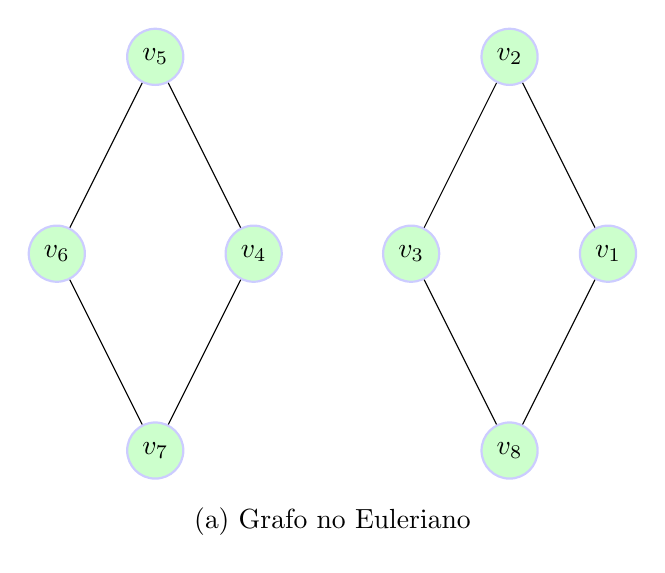
\begin{tikzpicture}{node distance=1.3cm,>=stealth',bend angle=45, auto}
  \tikzstyle{place}=[circle,thick,draw=blue!20,fill=green!20,minimum size=6mm]
  \tikzstyle{texto}=[]

  \begin{scope}

    \node [place] (c1) [xshift=-20cm]{$v_6$};

    \node [place] (c2) [right of=c1,xshift=.25cm,yshift=2.5cm] {$v_5$}
    edge [] (c1);

    \node [place] (c3) [right of=c1,xshift=.25cm,yshift=-2.5cm] {$v_7$}
    edge [] (c1);

    \node [place] (c4) [right of=c1,xshift=1.5cm] {$v_4$}
    edge [] (c2)
    edge [] (c3);

    \node [place] (c5) [right of=c4,xshift=1cm] {$v_3$};

    \node [place] (c6) [right of=c5,xshift=.25cm,yshift=2.5cm] {$v_2$}
    edge [] (c5);

    \node [place] (c7) [right of=c5,xshift=.25cm,yshift=-2.5cm] {$v_8$}
    edge [] (c5);

    \node [place] (c8) [right of=c5,xshift=1.5cm] {$v_1$}
    edge [] (c6)
    edge [] (c7);

    \node [texto] (p1) [below of=c7,yshift=.1cm,xshift=-2.25cm] {(a) Grafo no Euleriano};
  \end{scope}
\end{tikzpicture}
\end{minipage}}
\hspace*{.2in}{ \begin{minipage}{3cm}
\begin{center}
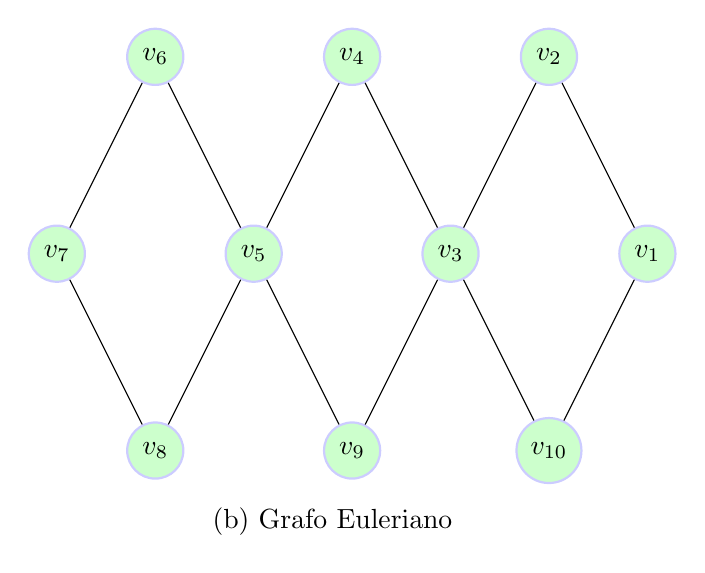
\begin{tikzpicture}{node distance=1.3cm,>=stealth',bend angle=45,auto}

  \tikzstyle{place}=[circle,thick,draw=blue!20,fill=green!20,minimum size=6mm]
  \tikzstyle{texto}=[]

  \begin{scope}


    \node [place] (t1) {$v_7$};

    \node [place] (t2) [right of=t1,xshift=.25cm,yshift=2.5cm] {$v_6$}
    edge [] (t1);

    \node [place] (t3) [right of=t1,xshift=.25cm,yshift=-2.5cm] {$v_8$}
    edge [] (t1);

    \node [place] (t4) [right of=t1,xshift=1.5cm] {$v_5$}
    edge [] (t2)
    edge [] (t3);

    \node [place] (t5) [right of=t4,xshift=1.5cm] {$v_3$};

    \node [place] (t6) [right of=t5,xshift=.25cm,yshift=2.5cm] {$v_2$}
    edge [] (t5);

    \node [place] (t7) [right of=t5,xshift=.25cm,yshift=-2.5cm] {$v_{10}$}
    edge [] (t5);

    \node [place] (t8) [right of=t5,xshift=1.5cm] {$v_1$}
    edge [] (t6)
    edge [] (t7);

    \node [place] (t9) [right of=t4,xshift=.25cm,yshift=2.5cm] {$v_4$}
    edge [] (t4)
    edge [] (t5);

    \node [place] (t10) [right of=t4,xshift=.25cm,yshift=-2.5cm] {$v_9$}
    edge [] (t4)
    edge [] (t5);

    \node [texto] (p1) [below of=t7,yshift=.1cm,xshift=-2.75cm] {(b) Grafo Euleriano};


\end{scope}  

\end{tikzpicture}

\end{center}
\end{minipage}}
\end{figure}
\end{center}

El grafo de la figura (a) nos muestra que la condición no es suficiente, es decir, existen grafos con todos los vértices de grado par y, sin embargo, no son eulerianos. Obsérvese que si \emph{conectamos} el grafo, entonces si es euleriano (apartado (b) de la figura). En efecto, el ciclo
\[ \gamma = \langle v_1, v_2, v_3, v_4, v_5, v_6, v_7, v_8, v_5, v_9, v_3, v_4, v_{10}, v_1 \rangle \]
es de Euler.\\

\begin{nota}
En el Primer Lema hemos visto que\\
\begin{center} Si $G$ es un Grafo Euleriano, entonces todos sus vértices son de grado par. \end{center}
de donde negando ambos miembros, y teniendo en cuenta la equivalencia lógica entre una proposición condicional y su contrarrecíproca, tendremos
\begin{center} Si existe algún vértice de grado impar, entonces $G$ no es Euleriano. \end{center}
es decir, si en un Grafo $G$ existe, al menos, un vértice de grado impar, entonces no es Euleriano.\\
\end{nota}

\subsection{Camino de Euler}

\begin{fondo}
Se dice que un camino de un grafo o multigrafo es de Euler si pasa por todos los vértices del mismo, recorriendo cada arista del mismo exactamente una vez.
\end{fondo}

Obsérvese que un \emph{camino de Euler} en un grafo $G$ puede entenderse también como una forma de dibujar el grafo sin levantar el lápiz del papel y sin pintar dos veces la misma arista.\\

\begin{nota}
El algoritmo implementado para el Camino de Euler comprueba la existencia de dicho camino o no. Hay otra versión que muestra en la salida estándar del sistema uno de los caminos posibles hallados.\\
\end{nota}

\underline{Camino de Euler}\\
\begin{Verbatim}[commandchars=\\\{\}]
\PY{c+cm}{/**}
\PY{c+cm}{ * Método observador (Euler dirigido)}
\PY{c+cm}{ * Método que llama al procedimiento general para la obtención del camino}
\PY{c+cm}{ * euleriano (si existe) del grafo euleriano (si lo es).}
\PY{c+cm}{ * @param G: matriz bidimensional de enteros cuyo contenido es el grafo}
\PY{c+cm}{ * de trabajo actual.}
\PY{c+cm}{ * @param v: valor entero que representa el nodo origen para el camino}
\PY{c+cm}{ * euleriano.}
\PY{c+cm}{ * @param w: valor entero que representa el nodo anterior procesado }
\PY{c+cm}{ * (en la primera llamada será el mismo nodo que v).}
\PY{c+cm}{ * @return boolean: devuelve true o fale si hay encontrado o no un }
\PY{c+cm}{ * camino euleriano para el grafo.}
\PY{c+cm}{ */}
    
\PY{k+kd}{public} \PY{k+kt}{boolean} \PY{n+nf}{camino\PYZus{}eulerGD}\PY{o}{(}\PY{k+kt}{int} \PY{o}{[}\PY{o}{]}\PY{o}{[}\PY{o}{]} \PY{n}{G}\PY{o}{,} \PY{k+kt}{int} \PY{n}{v}\PY{o}{,} \PY{k+kt}{int} \PY{n}{w}\PY{o}{)}
\PY{o}{\PYZob{}}
    \PY{n}{vert\PYZus{}orig\PYZus{}euler} \PY{o}{=} \PY{n}{w}\PY{o}{;}
    \PY{n}{algo\PYZus{}EulerGD}\PY{o}{(}\PY{n}{G}\PY{o}{,}\PY{n}{v}\PY{o}{,}\PY{n}{w}\PY{o}{)}\PY{o}{;}
	

    \PY{k}{return} \PY{n}{encontrado\PYZus{}euler}\PY{o}{;}
\PY{o}{\PYZcb{}}


\PY{c+cm}{/**}
\PY{c+cm}{ * Método modificador (Algoritmo Euler para grafos dirigidos)}
\PY{c+cm}{ * Un camino euleriano: un camino partiendo de un nodo origen que}
\PY{c+cm}{ * pase por todos los vértices (se pueden repetir) empleando todas}
\PY{c+cm}{ * las aristas posibles y regresando al nodo origen (ciclo).}
\PY{c+cm}{ * @param G: matriz bidimensional de enteros cuyo contenido es el grafo}
\PY{c+cm}{ * de trabajo actual.}
\PY{c+cm}{ * @param v: valor entero que representa el nodo origen para el camino}
\PY{c+cm}{ * euleriano.}
\PY{c+cm}{ * @param w: valor entero que representa el nodo anterior procesado }
\PY{c+cm}{ * (en la primera llamada será el mismo nodo que v).}
\PY{c+cm}{ */}

\PY{k+kd}{private} \PY{k+kt}{void} \PY{n+nf}{algo\PYZus{}EulerGD}\PY{o}{(}\PY{k+kt}{int} \PY{o}{[}\PY{o}{]}\PY{o}{[}\PY{o}{]} \PY{n}{G}\PY{o}{,} \PY{k+kt}{int} \PY{n}{v}\PY{o}{,} \PY{k+kt}{int} \PY{n}{w}\PY{o}{)}
\PY{o}{\PYZob{}}
    \PY{n}{grado\PYZus{}vector}\PY{o}{(}\PY{n}{G}\PY{o}{)}\PY{o}{;}
    \PY{k+kt}{int} \PY{n}{tama\PYZus{}G} \PY{o}{=} \PY{n}{G}\PY{o}{.}\PY{n+na}{length}\PY{o}{;}
    \PY{k+kt}{int} \PY{n}{t} \PY{o}{=} \PY{n}{grado\PYZus{}euler}\PY{o}{[}\PY{n}{v}\PY{o}{]} \PY{o}{+} \PY{n}{grado\PYZus{}euler}\PY{o}{[}\PY{n}{w}\PY{o}{]}\PY{o}{;}
    \PY{n}{dirigido\PYZus{}euler} \PY{o}{=} \PY{k+kc}{true}\PY{o}{;}

    \PY{n}{v\PYZus{}euler} \PY{o}{=} \PY{n}{v}\PY{o}{;}
    \PY{n}{pila\PYZus{}euler} \PY{o}{=} \PY{k}{new} \PY{n}{Stack}\PY{o}{<}\PY{n}{Integer}\PY{o}{>}\PY{o}{(}\PY{o}{)}\PY{o}{;}
    \PY{n}{hash\PYZus{}euler} \PY{o}{=} \PY{k}{new} \PY{n}{HashMap}\PY{o}{<}\PY{n}{Integer}\PY{o}{,}\PY{n}{ArrayList}\PY{o}{<}\PY{n}{Integer}\PY{o}{>}\PY{o}{>}\PY{o}{(}\PY{o}{)}\PY{o}{;}
    \PY{n}{ArrayList}\PY{o}{<}\PY{n}{Integer}\PY{o}{>} \PY{n}{adyacencias}\PY{o}{;}

    \PY{k}{for}\PY{o}{(}\PY{k+kt}{int} \PY{n}{i}\PY{o}{=}\PY{l+m+mi}{0}\PY{o}{;} \PY{n}{i} \PY{o}{<} \PY{n}{tama\PYZus{}G}\PY{o}{;} \PY{o}{+}\PY{o}{+}\PY{n}{i}\PY{o}{)}
	\PY{o}{\PYZob{}}
	    \PY{n}{adyacencias} \PY{o}{=} \PY{k}{new} \PY{n}{ArrayList}\PY{o}{<}\PY{n}{Integer}\PY{o}{>}\PY{o}{(}\PY{o}{)}\PY{o}{;}

	    \PY{k}{for}\PY{o}{(}\PY{k+kt}{int} \PY{n}{j}\PY{o}{=}\PY{l+m+mi}{0}\PY{o}{;} \PY{n}{j} \PY{o}{<} \PY{n}{tama\PYZus{}G}\PY{o}{;} \PY{o}{+}\PY{o}{+}\PY{n}{j}\PY{o}{)}
		\PY{o}{\PYZob{}}
		    \PY{k}{if}\PY{o}{(}\PY{n}{G}\PY{o}{[}\PY{n}{i}\PY{o}{]}\PY{o}{[}\PY{n}{j}\PY{o}{]} \PY{o}{!}\PY{o}{=} \PY{l+m+mi}{0}\PY{o}{)}
			\PY{o}{\PYZob{}}

			    \PY{n}{adyacencias}\PY{o}{.}\PY{n+na}{add}\PY{o}{(}\PY{n}{j}\PY{o}{)}\PY{o}{;}
			\PY{o}{\PYZcb{}}
		\PY{o}{\PYZcb{}}

	    \PY{n}{hash\PYZus{}euler}\PY{o}{.}\PY{n+na}{put}\PY{o}{(}\PY{n}{i}\PY{o}{,}\PY{n}{adyacencias}\PY{o}{)}\PY{o}{;}
	\PY{o}{\PYZcb{}}

    \PY{n}{encontrado\PYZus{}euler} \PY{o}{=} \PY{n}{entrada\PYZus{}salida\PYZus{}euler}\PY{o}{(}\PY{n}{G}\PY{o}{.}\PY{n+na}{length}\PY{o}{)}\PY{o}{;}

\PY{o}{\PYZcb{}}
\end{Verbatim}


\subsection{Segundo lema}

\begin{fondo}
Una condición necesaria para que un grafo o multigrafo admita un camino de Euler es que el número de vértices de grado impar sea 2 o ninguno.
\end{fondo}

\underline{Demostración}\\

Sea $G = (V,A)$ un grafo con un camino de Euler $\gamma = \langle u, u_1, u_2, \ldots, u_p, v \rangle$. \\
Tomamos un punto $w$ que no pertenezca a $V$ y sea $G' = (V',A')$ un grafo tal que
\[V' = V \cup \{w\} \]
\[ A' = A \cup \{uw, vw\} \]
es decir, el grafo obtenido añadiendo el nuevo punto como vértice al grafo original y las dos aristas adyacentes al mismo y a los extremos $u$ y $v$.\\
El ciclo
\[ \langle w, u, u_1, \ldots, u_p, v, w \rangle \]
es de Euler en $G'$, de aquí que $G'$ sea un grafo euleriano y aplicando el \emph{primer lema}, tengamos que todos sus vértices son de grado par.\\
Pues bien, si $x$ es cualquier vértice de $G$ distinto de $u$ y de $v$, entonces
\[ gr_G(x) = gr_{G'}(x) \]
luego el grado de $x$ en el grafo $G$ es par. Por otra parte,
\[ \begin{array}{l c}
  & gr_G(u) = gr_{G'}(u) - 1 \Longrightarrow gr_G(u)\ \mbox{es impar} \\
  \mbox{y} &\\
  & gr_G(v) = gr_{G'}(v) - 1 \Longrightarrow gr_G(v)\ \mbox{es impar}
\end{array} \]

luego los únicos dos vértices de grado impar son $u$ y $v$.\\

\begin{nota}
En el segundo lema, hemos visto que
\begin{quote}
\emph{``Si $G$ es un grafo con un camino de Euler, entonces el número de vértices de grado impar es 2 o ninguno''}
\end{quote}
Si ahora negamos ambos miembros, y tenemos en cuenta la equivalencia lógica entre una proposición condicional y su contrarrecíproca, tendremos
\begin{quote}
\emph{``Si el número de vértices de grado impar es distinto de 2, entonces $G$ no tiene ningún camino de Euler''}
\end{quote}
\end{nota}

\subsection{Tercer lema}

\begin{fondo}
Si $G$ es un grafo en el que todos sus vértices tienen grado par, entonces para cada par de vértices adyacentes de $G$, puede encontrarse un ciclo que contiene a la arista que forman ambos.
\end{fondo}

\underline{Demostración}\\
\\
Sean $u$ y $v$ dos vértices adyacentes de $G$ y sea $\gamma$ un camino que comienza en $u$ y continúa por la arista $uv$.\\
\\
Cada vez que $\gamma$ llega a un vértice $w$ distinto de $u$, continuamos el camino por una arista que no esté en $\gamma$, si $w$ es igual a $u$ damos por terminado el proceso. Dado que los grados de los vértices son pares por hipótesis, cada vez que el camino $\gamma$ pasa por un vértice utiliza dos aristas con un extremo en el mismo. Como el número de aristas y el de vértices es finito, el camino $\gamma$ acaba por volver a $u$ y $\gamma$ es, según la construcción hecha, un ciclo. \\


\section{Caminos y ciclos de Hamilton}

Se dice que el matemático irlandés William Hamilton (1805-1865) en el año 1857 inventó un juego que consistía en buscar un recorrido que diera la vuelta al mundo, representado por un dodecaedro, visitando cada ciudad, correspondiente a un vértice del dodecaedro, una sola vez. Solamente se podía desplazar de una ciudad a otra si los vértices correspondientes del dodecaedro estaban unidos por una arista.\\

El problema de decisión consistente en determinar si un grafo es hamiltoniano (contiene un ciclo que pasa una sola vez por cada vértice) es un problema de la clase NP-completo. \ref{sec:NP-section}

\subsection{Ciclo de Hamilton}

\begin{fondo}
Un ciclo simple en un grafo o multigrafo $G$ se dice que es de Hamilton, si contiene a todos los vértices de $G$.
\end{fondo}

\subsection{Grafo hamiltoniano}

\begin{fondo}
Un grafo o multigrafo que contenga un ciclo de Hamilton se denomina Hamiltoniano.
\end{fondo}

Para que un grafo sea Hamiltoniano deberá de cumplir las siguientes condiciones necesarias:\\
\begin{itemize}
\item Si un grafo $G = (V,A)$ es hamiltoniano entonces es conexo.
\item Si un grafo $G = (V,A)$ es hamiltoniano entonces $gr_G(V) \geq 2$.
\item Si un grafo $G = (V,A)$ es hamiltoniano entonces es conexo y no tiene vértices o puntos de corte.
\end{itemize}

Además deberá cumplir la siguiente condición suficiente:\\
\begin{itemize}
\item \underline{Teorema de Dirac}: Si un grafo $G = (V,A)$ de $n$ vértices (siendo $n \geq 3$) verifica que $gr_G(V) \geq n/2$ entonces es hamiltoniano.
\end{itemize}

\subsection{Camino de Hamilton}

\begin{fondo}
Un camino simple en un grafo o multigrafo $G$ que contenga a todos los vértices se denomina camino de Hamilton.
\end{fondo}

Para que un grafo posea un Camino Hamiltoniano deberá de cumplir las siguientes condiciones necesarias:\\
\begin{itemize}
\item Si un grafo $G = (V,A)$ admite un camino hamiltoniano entonces es conexo.
\item Si un grafo $G = (V,A)$ admite un camino hamiltoniano entonces no puede haber más de dos vértices con valencia no superior a 1.
\item Si un grafo $G = (V,A)$ admite un camino hamiltoniano entonces no puede tener un vértice de corte cuya eliminación de lugar a más de dos componentes conexas.
\end{itemize}

Además deberá cumplir la siguiente condición suficiente:\\
\begin{itemize}
\item Si un grafo $G = (V,A)$ de n vértices ($n \geq 3$) verifica que $gr_G(V) \geq (n-1)/2$ entonces admite un camino hamiltoniano.
\end{itemize}

\underline{Camino de Hamilton}\\
\begin{Verbatim}[commandchars=\\\{\}]
\PY{c+cm}{/**}
\PY{c+cm}{ * Método observador (Camino Hamiltoniano)}
\PY{c+cm}{ * Un grafo dirigido tendrá un camino Hamiltoniano }
\PY{c+cm}{ * (será grafo hamiltoniano) si existe un vértice que partiendo desde él }
\PY{c+cm}{ * se pase por cada vértice restante del grafo, una sola vez por nodo, y }
\PY{c+cm}{ * volviendo exactamente al nodo de partida.}
\PY{c+cm}{ * @param G: matriz bidimensional de enteros que representa al grafo}
\PY{c+cm}{ * de trabajo.}
\PY{c+cm}{ * @param v: valor entero que representa el nodo de partida para el }
\PY{c+cm}{ * camino.}
\PY{c+cm}{ * @param w: valor entero que representa el nodo anterior visitado.}
\PY{c+cm}{ */}

\PY{k+kd}{public} \PY{k+kt}{void} \PY{n+nf}{algo\PYZus{}Hamilton}\PY{o}{(}\PY{k+kt}{int} \PY{o}{[}\PY{o}{]}\PY{o}{[}\PY{o}{]} \PY{n}{G}\PY{o}{,} \PY{k+kt}{int} \PY{n}{v}\PY{o}{,} \PY{k+kt}{int} \PY{n}{w}\PY{o}{)}
\PY{o}{\PYZob{}}
    \PY{k+kt}{int} \PY{n}{tam\PYZus{}G} \PY{o}{=} \PY{n}{G}\PY{o}{.}\PY{n+na}{length}\PY{o}{;}
    \PY{n}{visitado\PYZus{}hamilton} \PY{o}{=} \PY{k}{new} \PY{k+kt}{boolean}\PY{o}{[}\PY{n}{tam\PYZus{}G}\PY{o}{]}\PY{o}{;}
    \PY{n}{Arrays}\PY{o}{.}\PY{n+na}{fill}\PY{o}{(}\PY{n}{visitado\PYZus{}hamilton}\PY{o}{,}\PY{k+kc}{false}\PY{o}{)}\PY{o}{;}
    \PY{n}{pila\PYZus{}hamilton} \PY{o}{=} \PY{k}{new} \PY{n}{Stack}\PY{o}{<}\PY{n}{Integer}\PY{o}{>}\PY{o}{(}\PY{o}{)}\PY{o}{;}
    \PY{n}{origen\PYZus{}hamilton} \PY{o}{=} \PY{n}{v}\PY{o}{;}

    \PY{k+kt}{boolean} \PY{n}{encontrado} \PY{o}{=} \PY{n}{algo\PYZus{}HamiltonRec}\PY{o}{(}\PY{n}{v}\PY{o}{,}\PY{n}{w}\PY{o}{,}\PY{n}{G}\PY{o}{,}\PY{n}{tam\PYZus{}G}\PY{o}{)}\PY{o}{;}

    \PY{k}{if}\PY{o}{(}\PY{n}{encontrado}\PY{o}{)}
	\PY{o}{\PYZob{}}
	    \PY{n}{Stack}\PY{o}{<}\PY{n}{Integer}\PY{o}{>} \PY{n}{salida\PYZus{}hamilton} \PY{o}{=} \PY{k}{new} \PY{n}{Stack}\PY{o}{<}\PY{n}{Integer}\PY{o}{>}\PY{o}{(}\PY{o}{)}\PY{o}{;}
		
	    \PY{k}{while}\PY{o}{(}\PY{o}{!}\PY{n}{pila\PYZus{}hamilton}\PY{o}{.}\PY{n+na}{empty}\PY{o}{(}\PY{o}{)}\PY{o}{)}
		\PY{o}{\PYZob{}}
		    \PY{n}{salida\PYZus{}hamilton}\PY{o}{.}\PY{n+na}{push}\PY{o}{(}\PY{n}{pila\PYZus{}hamilton}\PY{o}{.}\PY{n+na}{peek}\PY{o}{(}\PY{o}{)}\PY{o}{)}\PY{o}{;}
		    \PY{n}{pila\PYZus{}hamilton}\PY{o}{.}\PY{n+na}{pop}\PY{o}{(}\PY{o}{)}\PY{o}{;}
		\PY{o}{\PYZcb{}}

	    \PY{n}{System}\PY{o}{.}\PY{n+na}{out}\PY{o}{.}\PY{n+na}{print}\PY{o}{(}\PY{l+s}{"("}\PY{o}{)}\PY{o}{;}
	    \PY{k}{while}\PY{o}{(}\PY{o}{!}\PY{n}{salida\PYZus{}hamilton}\PY{o}{.}\PY{n+na}{empty}\PY{o}{(}\PY{o}{)}\PY{o}{)}
		\PY{o}{\PYZob{}}
		    \PY{n}{System}\PY{o}{.}\PY{n+na}{out}\PY{o}{.}\PY{n+na}{print}\PY{o}{(}\PY{l+s}{" "}\PY{o}{+}\PY{n}{salida\PYZus{}hamilton}\PY{o}{.}\PY{n+na}{peek}\PY{o}{(}\PY{o}{)}\PY{o}{)}\PY{o}{;}
		    \PY{n}{salida\PYZus{}hamilton}\PY{o}{.}\PY{n+na}{pop}\PY{o}{(}\PY{o}{)}\PY{o}{;}
		\PY{o}{\PYZcb{}}
	    \PY{n}{System}\PY{o}{.}\PY{n+na}{out}\PY{o}{.}\PY{n+na}{println}\PY{o}{(}\PY{l+s}{" )"}\PY{o}{)}\PY{o}{;}
	
	\PY{o}{\PYZcb{}}
    \PY{k}{else}
	\PY{n}{System}\PY{o}{.}\PY{n+na}{out}\PY{o}{.}\PY{n+na}{println}\PY{o}{(}\PY{l+s}{"No hay camino hamiltoniano para el grafo"}\PY{o}{)}\PY{o}{;}
\PY{o}{\PYZcb{}}

\PY{c+cm}{/**}
\PY{c+cm}{ * Método observador. (privado)}
\PY{c+cm}{ * Método que realiza el cálculo recursivo sobre los nodos necesarios}
\PY{c+cm}{ * del grafo.}
\PY{c+cm}{ * @param v: valor entero que representa el nodo actual. }
\PY{c+cm}{ * @param w: valor entero que representa el nodo anterior procesado.}
\PY{c+cm}{ * @param G: matriz bidimensional de enteros que representa el grafo de }
\PY{c+cm}{ * trabajo actual.}
\PY{c+cm}{ * @param d: valor entero que representa el número de nodos del grafo.}
\PY{c+cm}{ */}

\PY{k+kd}{private} \PY{k+kt}{boolean} \PY{n+nf}{algo\PYZus{}HamiltonRec}\PY{o}{(}\PY{k+kt}{int} \PY{n}{v}\PY{o}{,} \PY{k+kt}{int} \PY{n}{w}\PY{o}{,} \PY{k+kt}{int} \PY{o}{[}\PY{o}{]}\PY{o}{[}\PY{o}{]} \PY{n}{G}\PY{o}{,} \PY{k+kt}{int} \PY{n}{d}\PY{o}{)}
\PY{o}{\PYZob{}}
    \PY{k+kt}{int} \PY{n}{auxiliar} \PY{o}{=} \PY{l+m+mi}{0}\PY{o}{;}

    \PY{n}{visitado\PYZus{}hamilton}\PY{o}{[}\PY{n}{v}\PY{o}{]} \PY{o}{=} \PY{k+kc}{true}\PY{o}{;}
    \PY{n}{pila\PYZus{}hamilton}\PY{o}{.}\PY{n+na}{push}\PY{o}{(}\PY{n}{v}\PY{o}{)}\PY{o}{;} 
    \PY{c+c1}{//Tengo esta pila para luego rehacer el recorrido.}

    \PY{k}{for}\PY{o}{(}\PY{k+kt}{int} \PY{n}{j}\PY{o}{=}\PY{l+m+mi}{0}\PY{o}{;} \PY{n}{j} \PY{o}{<} \PY{n}{visitado\PYZus{}hamilton}\PY{o}{.}\PY{n+na}{length}\PY{o}{;} \PY{o}{+}\PY{o}{+}\PY{n}{j}\PY{o}{)}
	\PY{k}{if}\PY{o}{(}\PY{n}{visitado\PYZus{}hamilton}\PY{o}{[}\PY{n}{j}\PY{o}{]}\PY{o}{)}
	    \PY{n}{auxiliar}\PY{o}{+}\PY{o}{+}\PY{o}{;}

    \PY{k}{if}\PY{o}{(}\PY{n}{auxiliar} \PY{o}{=}\PY{o}{=} \PY{n}{visitado\PYZus{}hamilton}\PY{o}{.}\PY{n+na}{length}\PY{o}{)}
	\PY{k}{if}\PY{o}{(}\PY{n}{G}\PY{o}{[}\PY{n}{v}\PY{o}{]}\PY{o}{[}\PY{n}{origen\PYZus{}hamilton}\PY{o}{]} \PY{o}{=}\PY{o}{=} \PY{l+m+mi}{1} \PY{o}{&}\PY{o}{&} \PY{n}{d}\PY{o}{-}\PY{l+m+mi}{1} \PY{o}{=}\PY{o}{=} \PY{l+m+mi}{0}\PY{o}{)}
	    \PY{o}{\PYZob{}}
		\PY{n}{pila\PYZus{}hamilton}\PY{o}{.}\PY{n+na}{push}\PY{o}{(}\PY{n}{origen\PYZus{}hamilton}\PY{o}{)}\PY{o}{;}
		\PY{k}{return} \PY{k+kc}{true}\PY{o}{;}
	    \PY{o}{\PYZcb{}}



    \PY{k}{for}\PY{o}{(}\PY{k+kt}{int} \PY{n}{i} \PY{o}{=} \PY{l+m+mi}{0}\PY{o}{;} \PY{n}{i} \PY{o}{<} \PY{n}{G}\PY{o}{.}\PY{n+na}{length}\PY{o}{;} \PY{o}{+}\PY{o}{+}\PY{n}{i}\PY{o}{)}
	\PY{k}{if}\PY{o}{(}\PY{n}{G}\PY{o}{[}\PY{n}{v}\PY{o}{]}\PY{o}{[}\PY{n}{i}\PY{o}{]} \PY{o}{!}\PY{o}{=} \PY{l+m+mi}{0} \PY{o}{&}\PY{o}{&} \PY{o}{!}\PY{n}{visitado\PYZus{}hamilton}\PY{o}{[}\PY{n}{i}\PY{o}{]}\PY{o}{)}
	    \PY{k}{if}\PY{o}{(}\PY{n}{algo\PYZus{}HamiltonRec}\PY{o}{(}\PY{n}{i}\PY{o}{,}\PY{n}{v}\PY{o}{,}\PY{n}{G}\PY{o}{,}\PY{n}{d}\PY{o}{-}\PY{l+m+mi}{1}\PY{o}{)}\PY{o}{)}
		\PY{k}{return} \PY{k+kc}{true}\PY{o}{;}

    \PY{n}{pila\PYZus{}hamilton}\PY{o}{.}\PY{n+na}{pop}\PY{o}{(}\PY{o}{)}\PY{o}{;}
    \PY{n}{visitado\PYZus{}hamilton}\PY{o}{[}\PY{n}{v}\PY{o}{]} \PY{o}{=} \PY{k+kc}{false}\PY{o}{;}
    \PY{k}{return} \PY{k+kc}{false}\PY{o}{;}
\PY{o}{\PYZcb{}}
\end{Verbatim}


\begin{ejem}
El grafo de Peterson contiene un camino de Hamilton que comienza en cada uno de sus vértices. Este grafo es la base de la mayoría de los contraejemplos en las conjeturas sobre grafos de Hamilton.\\
\end{ejem}

\figuratikz{1}{Grafo de Peterson}
{
  \tikzstyle{place}=[circle,thick,draw=blue!20,fill=green!20,minimum size=4mm]
  \tikzstyle{texto}=[]

  \begin{scope}


    \node [place] (c1) {};

    \node [place] (c2) [right of=c1,xshift=1.5cm,yshift=2cm] {};

    \node [place] (c3) [right of=c1,xshift=4cm] {}
    edge [] (c1);

    \node [place] (c4) [right of=c1,yshift=-3.5cm,xshift=-.5cm] {}
    edge [] (c2)
    edge [] (c3);


    \node [place] (c5) [left of=c3,yshift=-3.5cm,xshift=.5cm] {}
    edge [] (c1)
    edge [] (c2);

    \node [place] (c6) [above of=c2,yshift=.5cm] {}
    edge [] (c2);

    \node [place] (c7) [below of=c4,yshift=-.2cm,xshift=-1.2cm] {}
    edge [] (c4);

    \node [place] (c8) [left of=c1,yshift=.5cm,xshift=-1.2cm] {}
    edge [] (c1)
    edge [] (c7)
    edge [] (c6);

    \node [place] (c9) [below of=c5,yshift=-.2cm,xshift=1.2cm] {}
    edge [] (c7)
    edge [] (c5);

    \node [place] (c10) [right of=c3,yshift=.5cm,xshift=1.2cm] {}
    edge [] (c6)
    edge [] (c9)
    edge [] (c3);

    
\end{scope}  

}

\section{Grafos ponderados}

\subsection{Caminos más cortos desde un vértice: Dijkstra}

El algoritmo de Dijkstra, aplicado a un (di)grafo ponderado con pesos no negativos (no funciona para pesos negativos, en cuyo caso hay que utilizar otro procedimiento llamada algoritmo (BELLMAN-FORD)[\ref{sec:bellman}], se fundamenta en algo evidente: si se pretende encontrar la distancia más corta desde un punto $A$ a otros puntos, y en un momento determinado se sabe la distancia más corta desde $A$ a un punto $D$, entonces se puede tratar de mejorar las distancias parciales conocidas desde $A$ a los vértices adyacentes a $D$ comparándolas con las distancias que se obtienen yendo desde $A$ a $D$ y desde $D$ a estos vértices, tal como ilustra la siguiente Figura.\\

\figuratikz{1}{Se cotejan las distancias desde el vértice base $D$}
{
  \tikzstyle{place}=[circle,thick,draw=blue!20,fill=green!20,minimum size=6mm]
  \tikzstyle{texto}=[]

  \begin{scope}


    \node [place] (c1) [label=left:$A$]{};

    \node [place] (c2) [right of=c1,yshift=1cm,xshift=.5cm] {}
    edge [dotted] (c1);

    \node [place] (c3) [right of=c2,yshift=2cm] {}
    edge [dotted] (c1);

    \node [place] (c4) [right of=c1,xshift=2cm,label=right:$D$] {}
    edge [densely dotted] (c1)
    edge [dashed] (c3)
    edge [dashed] (c2);

    \node [place]  (c5) [left of=c4,yshift=-1cm,xshift=-.5cm] {}
    edge [dashed] (c4)
    edge [densely dotted] (c1);

    \node [place]  (c6) [right of=c4,yshift=-1cm] {}
    edge [dashed] (c4);



\end{scope}  
}
La cristalización matemática de esta idea consiste en lo siguiente. Se define una función $l(x)$ que a cada vértice $x$ le asocie la distancia parcial conocida desde el vértice origen prefijado (llamémoslo $A$, por comodidad) hasta el propio vértice $x$. En cada etapa, cuando se haya determinado la distancia exacta de $A$ a un vértice $D$, el cual ejerce las labores de nueva base o pivote, se actualizan los valores $l(y)$ para vértices $y$ adyacentes a $D$ según la fórmula $l(y) =$ min$\{l(y),l(D)\ +\ peso(\{D,y\})\}$; de manera que si el camino desde $A$ hasta $D$ más la arista que va de $D$ a $y$ resulta más económico (esto es, más corto) que el que antes se conocía yendo desde $A$ hasta $y$ sin pasar por $D$ (distancia que marcaba el valor $l(y)$), se actualizaba el valor de $l(y)$ según el nuevo camino. A la hora de poder reconstruir los caminos que dan las distancias más cortas desde $A$, es necesario asimismo guardar la arista $\{D, y\}$ por la que se llega al vértice $y$.\\

En definitiva, el algoritmo de Dijkstra funciona así:\\
\begin{enumerate}
\item Se toma el vértice $A$ desde el que se van a hallar las distancias más cortas a los restantes vértices.
\item Se inicializan los valores $l(x)$ a infinito, para $x \neq A$, y $l(A) = 0$.
\item Se toma como primer vértice base (o pivote) a $A$, que será asimismo el vértice raíz del árbol recubridor que dará las distancias más cortas hasta $A$.
\item Ahora, utilizando $A$ como vértice base, se actualizan los valores $l(x)$ de aquellos vértices adyacentes a $A$ según la fórmula $l(x) =$ min$\{l(x),l(A)\ +\ peso(\{A,x\})\}$.
\item Se toma como nuevo vértice base uno de entre aquellos cuyas distancias a $A$ sea mínima, y se almacena la arista por la que se ha llegado a dicho vértice.
\item Sucesivamente, utilizando el vértice base $D$ correspondiente, se actualizan los valores $l(x)$ de aquellos vértices adyacentes a $D$ según la fórmula $l(x) =$ min $\{l(x),l(D)\ +\ peso(\{D,x\})\}$; de manera que se puede elegir al nuevo vértice base y la arista mediante la cual se ha llegado al mismo.
\item El proceso termina cuando ya se ha calculado las distancias más cortas a todos los vértices, requiriendo tantas etapas como vértices tiene el grafo menos 1.
\end{enumerate}

\figuratikz{1}{Un grafo dirigido ponderado y los pasos que realiza el algoritmo de Dijkstra en el grafo. En cada paso se colorean los nuevos vértices y las nuevas aristas procesadas.}
{
  \tikzstyle{place}=[circle,thick,draw=blue!20,fill=green!20,minimum size=5mm]
  \tikzstyle{texto}=[]
  \tikzstyle{process}=[circle,thick,draw=blue!20,fill=red!20,minimum size=5mm]

  \begin{scope}


    \node [place] (c1) {$v_5$};

    \node [process] (c2) [right of=c1,xshift=.5cm,yshift=2cm] {$v_1$}
    edge [post] node [above,xshift=-.2cm] {$1$} (c1);

    \node [place] (c3) [right of=c1,xshift=2cm] {$v_2$}
    edge [pre] node [above,xshift=.2cm] {$7$} (c2);

    \node [place] (c4) [below of=c1,xshift=.4cm,yshift=-.6cm] {$v_4$}
    edge [pre] node [below,yshift=.2cm,xshift=-.3cm] {$1$} (c1) 
    edge [pre] node [above,xshift=.3cm] {$6$} (c2)
    edge [post]  node [above] {$3$} (c3);

    \node [place] (c5) [below of=c3,xshift=-.4cm,yshift=-.6cm]  {$v_3$}
    edge [pre] node [above,xshift=-.3cm] {$4$} (c2)
    edge [post] node [below] {$5$} (c4)
    edge [post] node [below,yshift=.1cm,xshift=.3cm] {$2$} (c3) ;

    \node [process] (d1) [right of=c3,xshift=.2cm] {$v_5$};

    \node [process] (d2) [right of=d1,xshift=.5cm,yshift=2cm] {$v_1$}
    edge [red,post] node [above,xshift=-.2cm] {\textcolor{black}{$1$}} (d1);

    \node [place] (d3) [right of=d1,xshift=2cm] {$v_2$}
    edge [pre] node [above,xshift=.2cm] {$7$} (d2);

    \node [place] (d4) [below of=d1,xshift=.4cm,yshift=-.6cm] {$v_4$}
    edge [pre] node [below,yshift=.2cm,xshift=-.3cm] {$1$} (d1) 
    edge [pre] node [above,xshift=.3cm] {$6$} (d2)
    edge [post]  node [above] {$3$} (d3);

    \node [place] (d5) [below of=d3,xshift=-.4cm,yshift=-.6cm]  {$v_3$}
    edge [pre] node [above,xshift=-.3cm] {$4$} (d2)
    edge [post] node [below] {$5$} (d4)
    edge [post] node [below,yshift=.1cm,xshift=.3cm] {$2$} (d3) ;


    \node [process] (e1) [right of=d3,xshift=.2cm] {$v_5$};

    \node [process] (e2) [right of=e1,xshift=.5cm,yshift=2cm] {$v_1$}
    edge [red,post] node [above,xshift=-.2cm] {\textcolor{black}{$1$}} (e1);

    \node [place] (e3) [right of=e1,xshift=2cm] {$v_2$}
    edge [pre] node [above,xshift=.2cm] {$7$} (e2);

    \node [process] (e4) [below of=e1,xshift=.4cm,yshift=-.6cm] {$v_4$}
    edge [red,pre] node [below,yshift=.2cm,xshift=-.3cm] {\textcolor{black}{$1$}} (e1) 
    edge [pre] node [above,xshift=.3cm] {$6$} (e2)
    edge [post]  node [above] {$3$} (e3);

    \node [place] (e5) [below of=e3,xshift=-.4cm,yshift=-.6cm]  {$v_3$}
    edge [pre] node [above,xshift=-.3cm] {$4$} (e2)
    edge [post] node [below] {$5$} (e4)
    edge [post] node [below,yshift=.1cm,xshift=.3cm] {$2$} (e3) ;

    \node [process] (f1) [below of=c1,yshift=-3.5cm,xshift=2cm] {$v_5$};

    \node [process] (f2) [right of=f1,xshift=.5cm,yshift=2cm] {$v_1$}
    edge [red,post] node [above,xshift=-.2cm] {\textcolor{black}{$1$}} (f1);

    \node [place] (f3) [right of=f1,xshift=2cm] {$v_2$}
    edge [pre] node [above,xshift=.2cm] {$7$} (f2);

    \node [process] (f4) [below of=f1,xshift=.4cm,yshift=-.6cm] {$v_4$}
    edge [red,pre] node [below,yshift=.2cm,xshift=-.3cm] {\textcolor{black}{$1$}} (f1) 
    edge [pre] node [above,xshift=.3cm] {$6$} (f2)
    edge [post]  node [above] {$3$} (f3);

    \node [process] (f5) [below of=f3,xshift=-.4cm,yshift=-.6cm]  {$v_3$}
    edge [red,pre] node [above,xshift=-.3cm] {\textcolor{black}{$4$}} (f2)
    edge [post] node [below] {$5$} (f4)
    edge [post] node [below,yshift=.1cm,xshift=.3cm] {$2$} (f3) ;

    \node [process] (g1) [below of=d3,yshift=-3.5cm,xshift=-.8cm] {$v_5$};

    \node [process] (g2) [right of=g1,xshift=.5cm,yshift=2cm] {$v_1$}
    edge [red,post] node [above,xshift=-.2cm] {\textcolor{black}{$1$}} (g1);

    \node [process] (g3) [right of=g1,xshift=2cm] {$v_2$}
    edge [pre] node [above,xshift=.2cm] {$7$} (g2);

    \node [process] (g4) [below of=g1,xshift=.4cm,yshift=-.6cm] {$v_4$}
    edge [red,pre] node [below,yshift=.2cm,xshift=-.3cm] {\textcolor{black}{$1$}} (g1) 
    edge [pre] node [above,xshift=.3cm] {$6$} (g2)
    edge [red,post]  node [above] {\textcolor{black}{$3$}} (g3);

    \node [process] (g5) [below of=g3,xshift=-.4cm,yshift=-.6cm]  {$v_3$}
    edge [red,pre] node [above,xshift=-.3cm] {\textcolor{black}{$4$}} (g2)
    edge [post] node [below] {$5$} (g4)
    edge [post] node [below,yshift=.1cm,xshift=.3cm] {$2$} (g3) ;
    
\end{scope}  

}

\underline{Algoritmo de Dijkstra}\\
\begin{Verbatim}[commandchars=\\\{\}]
\PY{c+cm}{/**}
\PY{c+cm}{ * Método observador (Algoritmo de Dijkstra).}
\PY{c+cm}{ * Calcula los caminos de coste mínimo entre origen y }
\PY{c+cm}{ * todos los vértices del grafo G.}
\PY{c+cm}{ * @param origen vértice desde el que se realiza la computación.}
\PY{c+cm}{ * @param G matriz de costes asociada al grafo G.}
\PY{c+cm}{ * @return Un vector de tamaño G.length con estos costes }
\PY{c+cm}{ * mínimos (fila 0 de la matriz) y un vector de tamaño G.length }
\PY{c+cm}{ * tal que vector[i] es el último vértice del camino origen a i }
\PY{c+cm}{ * (fila 1 de la matriz).}
\PY{c+cm}{ * @exception Exception}
\PY{c+cm}{ */}

\PY{k+kd}{public} \PY{k+kt}{int}\PY{o}{[}\PY{o}{]}\PY{o}{[}\PY{o}{]} \PY{n+nf}{algo\PYZus{}Dijkstra}\PY{o}{(}\PY{k+kt}{int} \PY{n}{origen}\PY{o}{,} \PY{k+kt}{int} \PY{o}{[}\PY{o}{]}\PY{o}{[}\PY{o}{]} \PY{n}{G}\PY{o}{)} \PY{k+kd}{throws} \PY{n}{Exception}
\PY{o}{\PYZob{}}
    \PY{k+kt}{int} \PY{n}{tama\PYZus{}G}\PY{o}{=}\PY{n}{G}\PY{o}{.}\PY{n+na}{length}\PY{o}{;}

    \PY{c+cm}{/*}
\PY{c+cm}{      Voy a devolver como resultado de la función la variable definida }
\PY{c+cm}{      int [][] Costes\PYZus{}Vertices [2][G.length]. Donde la primera fila es }
\PY{c+cm}{      el vector de costes obtenido al aplicar Dijkstra y la segunda }
\PY{c+cm}{      fila es el vector obtenido del recorrido según se obtienen los }
\PY{c+cm}{      caminos mas cortos a partir del origen. }
\PY{c+cm}{    */}

    \PY{k+kt}{int} \PY{o}{[}\PY{o}{]}\PY{o}{[}\PY{o}{]} \PY{n}{Costes\PYZus{}Vertices} \PY{o}{=} \PY{k}{new} \PY{k+kt}{int}\PY{o}{[}\PY{l+m+mi}{2}\PY{o}{]}\PY{o}{[}\PY{n}{tama\PYZus{}G}\PY{o}{]}\PY{o}{;}

    \PY{k+kt}{boolean} \PY{o}{[}\PY{o}{]} \PY{n}{Visitado} \PY{o}{=} \PY{k}{new} \PY{k+kt}{boolean}\PY{o}{[}\PY{n}{tama\PYZus{}G}\PY{o}{]}\PY{o}{;}
    \PY{k+kt}{int} \PY{n}{i}\PY{o}{;}
    \PY{k+kt}{int} \PY{n}{v}\PY{o}{,}\PY{n}{w}\PY{o}{=}\PY{l+m+mi}{0}\PY{o}{;}
    \PY{k+kt}{int} \PY{n}{CosteMin}\PY{o}{,} \PY{n}{Owv}\PY{o}{;}
	
    \PY{c+cm}{/* Marcamos como visitado el origen. */}
    \PY{n}{Visitado}\PY{o}{[}\PY{n}{origen}\PY{o}{]} \PY{o}{=} \PY{k+kc}{true}\PY{o}{;}

    \PY{k}{for}\PY{o}{(}\PY{n}{v}\PY{o}{=}\PY{l+m+mi}{0}\PY{o}{;} \PY{n}{v} \PY{o}{<} \PY{n}{tama\PYZus{}G}\PY{o}{;} \PY{o}{+}\PY{o}{+}\PY{n}{v}\PY{o}{)}
	\PY{o}{\PYZob{}}
	    \PY{n}{Costes\PYZus{}Vertices}\PY{o}{[}\PY{l+m+mi}{0}\PY{o}{]}\PY{o}{[}\PY{n}{v}\PY{o}{]} \PY{o}{=} \PY{n}{G}\PY{o}{[}\PY{n}{origen}\PY{o}{]}\PY{o}{[}\PY{n}{v}\PY{o}{]}\PY{o}{;}

	    \PY{c+cm}{/*Asignamos todos los costes asociados partiendo desde}
\PY{c+cm}{	      el vertice origen. */}

	    \PY{n}{Costes\PYZus{}Vertices}\PY{o}{[}\PY{l+m+mi}{1}\PY{o}{]}\PY{o}{[}\PY{n}{v}\PY{o}{]} \PY{o}{=} \PY{n}{origen}\PY{o}{;}
	    \PY{c+c1}{//El vector tiene como elementos al vertice origen.}
	\PY{o}{\PYZcb{}}

    \PY{k}{for}\PY{o}{(}\PY{n}{i}\PY{o}{=}\PY{l+m+mi}{0}\PY{o}{;} \PY{n}{i} \PY{o}{<} \PY{n}{tama\PYZus{}G}\PY{o}{-}\PY{l+m+mi}{1}\PY{o}{;} \PY{o}{+}\PY{o}{+}\PY{n}{i}\PY{o}{)}
	\PY{o}{\PYZob{}}
	    \PY{c+cm}{/*Localizar vértice w no incluido en S con coste}
\PY{c+cm}{	      mínimo desde origen. */}
	    \PY{n}{CosteMin} \PY{o}{=} \PY{n}{Integer}\PY{o}{.}\PY{n+na}{MAX\PYZus{}VALUE}\PY{o}{;}

	    \PY{k}{for}\PY{o}{(}\PY{n}{v}\PY{o}{=}\PY{l+m+mi}{0}\PY{o}{;} \PY{n}{v} \PY{o}{<} \PY{n}{tama\PYZus{}G}\PY{o}{;}\PY{o}{+}\PY{o}{+}\PY{n}{v}\PY{o}{)}
		\PY{k}{if}\PY{o}{(}\PY{o}{!}\PY{n}{Visitado}\PY{o}{[}\PY{n}{v}\PY{o}{]} \PY{o}{&}\PY{o}{&} \PY{n}{Costes\PYZus{}Vertices}\PY{o}{[}\PY{l+m+mi}{0}\PY{o}{]}\PY{o}{[}\PY{n}{v}\PY{o}{]} \PY{o}{<} \PY{n}{CosteMin}\PY{o}{)}
		    \PY{o}{\PYZob{}}
			\PY{n}{CosteMin} \PY{o}{=} \PY{n}{Costes\PYZus{}Vertices}\PY{o}{[}\PY{l+m+mi}{0}\PY{o}{]}\PY{o}{[}\PY{n}{v}\PY{o}{]}\PY{o}{;}
			\PY{n}{w} \PY{o}{=} \PY{n}{v}\PY{o}{;}
		    \PY{o}{\PYZcb{}}

	    \PY{n}{Visitado}\PY{o}{[}\PY{n}{w}\PY{o}{]} \PY{o}{=} \PY{k+kc}{true}\PY{o}{;}

	    \PY{k}{for}\PY{o}{(}\PY{n}{v}\PY{o}{=}\PY{l+m+mi}{0}\PY{o}{;} \PY{n}{v} \PY{o}{<} \PY{n}{tama\PYZus{}G}\PY{o}{;}\PY{o}{+}\PY{o}{+}\PY{n}{v}\PY{o}{)}
		\PY{o}{\PYZob{}}
		    \PY{n}{Owv} \PY{o}{=} \PY{n}{Suma}\PY{o}{(}\PY{n}{Costes\PYZus{}Vertices}\PY{o}{[}\PY{l+m+mi}{0}\PY{o}{]}\PY{o}{[}\PY{n}{w}\PY{o}{]}\PY{o}{,}\PY{n}{G}\PY{o}{[}\PY{n}{w}\PY{o}{]}\PY{o}{[}\PY{n}{v}\PY{o}{]}\PY{o}{)}\PY{o}{;}

		    \PY{k}{if}\PY{o}{(}\PY{o}{!}\PY{n}{Visitado}\PY{o}{[}\PY{n}{v}\PY{o}{]} \PY{o}{&}\PY{o}{&} \PY{n}{Costes\PYZus{}Vertices}\PY{o}{[}\PY{l+m+mi}{0}\PY{o}{]}\PY{o}{[}\PY{n}{v}\PY{o}{]} \PY{o}{>} \PY{n}{Owv}\PY{o}{)}
			\PY{o}{\PYZob{}}
			    \PY{n}{Costes\PYZus{}Vertices}\PY{o}{[}\PY{l+m+mi}{0}\PY{o}{]}\PY{o}{[}\PY{n}{v}\PY{o}{]} \PY{o}{=} \PY{n}{Owv}\PY{o}{;}
			    \PY{n}{Costes\PYZus{}Vertices}\PY{o}{[}\PY{l+m+mi}{1}\PY{o}{]}\PY{o}{[}\PY{n}{v}\PY{o}{]} \PY{o}{=} \PY{n}{w}\PY{o}{;}
			\PY{o}{\PYZcb{}}
		\PY{o}{\PYZcb{}}
	\PY{o}{\PYZcb{}}

    \PY{k}{return} \PY{n}{Costes\PYZus{}Vertices}\PY{o}{;}
\PY{o}{\PYZcb{}}
\end{Verbatim}


\subsection{Caminos más cortos desde un vértice: Bellman-Ford}
\label{sec:bellman}

El algoritmo de Bellman-Ford resuelve el problema del camino más corto posible desde un vértice origen de un grafo en el caso general de que los pesos de las aristas puedan ser negativos. Dado un grafo ponderado y dirigido $G = (V,A)$ con un vértice origen $s$ y la función de coste o ponderación $w: A \rightarrow \mathbb{R}$, el algoritmo de Bellman-Ford devuelve un valor booleano que indica si existe o no un ciclo de coste negativo que fuera accesible desde el vértice origen. Si es que existe un ciclo, el algoritmo indica que no existe solución. Si no hay ciclo de este tipo, el algoritmo produce los caminos más cortos asociados a los pesos.\\

El algoritmo relaja las aristas que va procesando, disminuyendo progresivamente la estimación del peso del vértice a través de los caminos más cortos posibles desde $s$ a cada vértice $v \in V$ hasta que se logre el camino real de peso más corto. El algoritmo devuelve \textbf{true} si y sólo si el grafo no contiene ciclos de peso negativo que sean accesibles desde el vértice origen.\\

\vfill
\pagebreak

\figuratikz{1}{La ejecución del algoritmo de Bellman-Ford.}
{
  \tikzstyle{place}=[circle,thick,draw=blue!20,fill=green!20,minimum size=8mm]
  \tikzstyle{texto}=[]
  \tikzstyle{process}=[circle,thick,draw=blue!20,fill=red!20,minimum size=8mm]

  \begin{scope}


    \node [place] (c1) {$\infty$};

    \node [process] (c2) [right of=c1,xshift=.5cm,yshift=2cm] {$0$}
    edge [post] node [above,xshift=-.2cm] {$7$} (c1);

    \node [place] (c3) [right of=c1,xshift=2cm] {$\infty$}
    edge [pre] node [above,xshift=.2cm] {$6$} (c2)
    edge [post] node [above] {$8$} (c1);

    \node [place] (c4) [below of=c1,yshift=-.8cm] {$\infty$}
    edge [pre] node [below,xshift=-.2cm] {$9$} (c1)
    edge [pre] node [left,yshift=-.5cm] {$-4$} (c3)
    edge [post] node [above,yshift=.4cm,xshift=.5cm] {$2$} (c2);

    \node [place] (c5) [below of=c3,yshift=-.8cm]  {$\infty$}
    edge [pre] node [below] {$7$} (c4)
    edge [pre] node [left,yshift=.5cm] {$-3$} (c1)
    edge [pre,bend right] node [right] {$5$} (c3)
    edge [post,bend left] node [left] {$-2$} (c3);
 

    \node [process] (d1) [right of=c3,xshift=.5cm] {$7$};

    \node [place] (d2) [right of=d1,xshift=.5cm,yshift=2cm] {$0$}
    edge [post,red] node [above,xshift=-.2cm] {\textcolor{black}{$7$}} (d1);

    \node [process] (d3) [right of=d1,xshift=2cm] {$6$}
    edge [pre,red] node [above,xshift=.2cm] {\textcolor{black}{$6$}} (d2)
    edge [post] node [above] {$8$} (d1);

    \node [place] (d4) [below of=d1,yshift=-.8cm] {$\infty$}
    edge [pre] node [below,xshift=-.2cm] {$9$} (d1)
    edge [pre] node [left,yshift=-.5cm] {$-4$} (d3)
    edge [post] node [above,yshift=.4cm,xshift=.5cm] {$2$} (d2);

    \node [place] (d5) [below of=d3,yshift=-.8cm]  {$\infty$}
    edge [pre] node [below] {$7$} (d4)
    edge [pre] node [left,yshift=.5cm] {$-3$} (d1)
    edge [pre,bend right] node [right] {$5$} (d3)
    edge [post,bend left] node [left] {$-2$} (d3);


    \node [place] (e1) [right of=d3,xshift=.5cm] {$7$};

    \node [place] (e2) [right of=e1,xshift=.5cm,yshift=2cm] {$0$}
    edge [post,red] node [above,xshift=-.2cm] {\textcolor{black}{$7$}} (e1);

    \node [place] (e3) [right of=e1,xshift=2cm] {$6$}
    edge [pre,red] node [above,xshift=.2cm] {\textcolor{black}{$6$}} (e2)
    edge [post] node [above] {$8$} (e1);

    \node [process] (e4) [below of=e1,yshift=-.8cm] {$2$}
    edge [pre] node [below,xshift=-.2cm] {$9$} (e1)
    edge [pre,red] node [left,yshift=-.5cm] {\textcolor{black}{$-4$}} (e3)
    edge [post] node [above,yshift=.4cm,xshift=.5cm] {$2$} (e2);

    \node [process] (e5) [below of=e3,yshift=-.8cm]  {$4$}
    edge [pre] node [below] {$7$} (e4)
    edge [pre,red] node [left,yshift=.5cm] {\textcolor{black}{$-3$}} (e1)
    edge [pre,bend right] node [right] {$5$} (e3)
    edge [post,bend left] node [left] {\textcolor{black}{$-2$}} (e3);

    \node [place] (f1) [below of=c1,yshift=-5.5cm,xshift=2cm] {$7$};

    \node [place] (f2) [right of=f1,xshift=.5cm,yshift=2cm] {$0$}
    edge [post,red] node [above,xshift=-.2cm] {\textcolor{black}{$7$}} (f1);

    \node [process] (f3) [right of=f1,xshift=2cm] {$2$}
    edge [pre] node [above,xshift=.2cm] {$6$} (f2)
    edge [post] node [above] {$8$} (f1);

    \node [place] (f4) [below of=f1,yshift=-.8cm] {$2$}
    edge [pre] node [below,xshift=-.2cm] {$9$} (f1)
    edge [pre,red] node [left,yshift=-.5cm] {\textcolor{black}{$-4$}} (f3)
    edge [post] node [above,yshift=.4cm,xshift=.5cm] {$2$} (f2);

    \node [place] (f5) [below of=f3,yshift=-.8cm]  {$4$}
    edge [pre] node [below] {$7$} (f4)
    edge [pre,red] node [left,yshift=.5cm] {\textcolor{black}{$-3$}} (f1)
    edge [pre,bend right] node [right] {$5$} (f3)
    edge [post,bend left,red] node [left] {\textcolor{black}{$-2$}} (f3);


    \node [place] (g1) [below of=d3,yshift=-5.5cm,xshift=-.8cm] {$7$};

    \node [place] (g2) [right of=g1,xshift=.5cm,yshift=2cm] {$0$}
    edge [post,red] node [above,xshift=-.2cm] {\textcolor{black}{$7$}} (g1);

    \node [place] (g3) [right of=g1,xshift=2cm] {$2$}
    edge [pre] node [above,xshift=.2cm] {$6$} (g2)
    edge [post] node [above] {$8$} (g1);

    \node [process] (g4) [below of=g1,yshift=-.8cm] {$-2$}
    edge [pre] node [below,xshift=-.2cm] {$9$} (g1)
    edge [pre,red] node [left,yshift=-.5cm] {\textcolor{black}{$-4$}} (g3)
    edge [post] node [above,yshift=.4cm,xshift=.5cm] {$2$} (g2);

    \node [place] (g5) [below of=g3,yshift=-.8cm]  {$4$}
    edge [pre] node [below] {$7$} (g4)
    edge [pre,red] node [left,yshift=.5cm] {\textcolor{black}{$-3$}} (g1)
    edge [pre,bend right] node [right] {$5$} (g3)
    edge [post,bend left,red] node [left] {\textcolor{black}{$-2$}} (g3);

\end{scope}  

}

\underline{Algoritmo de Bellman-Ford}\\
\begin{Verbatim}[commandchars=\\\{\}]
\PY{c+cm}{/**}
\PY{c+cm}{ * Procedimiento de Bellman-Ford (llamada al algoritmo principal)}
\PY{c+cm}{ * @param G: matriz de costes del grafo conexo G.}
\PY{c+cm}{ * @param x: valor entero que representa el nodo origen.}
\PY{c+cm}{ * @return void}
\PY{c+cm}{ */}

\PY{k+kd}{public} \PY{k+kt}{void} \PY{n+nf}{Bellman\PYZus{}Ford} \PY{o}{(}\PY{k+kt}{int} \PY{o}{[}\PY{o}{]}\PY{o}{[}\PY{o}{]} \PY{n}{G}\PY{o}{,} \PY{k+kt}{int} \PY{n}{x}\PY{o}{)}
\PY{o}{\PYZob{}}
    \PY{n}{System}\PY{o}{.}\PY{n+na}{out}\PY{o}{.}\PY{n+na}{println}\PY{o}{(}\PY{l+s}{"BELLMAN-FORD"}\PY{o}{)}\PY{o}{;}

    \PY{k+kt}{int} \PY{n}{i}\PY{o}{;}
	
    \PY{k}{if}\PY{o}{(}\PY{n}{algo\PYZus{}Bellman\PYZus{}Ford}\PY{o}{(}\PY{n}{G}\PY{o}{,}\PY{n}{x}\PY{o}{)} \PY{o}{=}\PY{o}{=} \PY{k+kc}{true}\PY{o}{)}
	\PY{o}{\PYZob{}}
	    \PY{n}{System}\PY{o}{.}\PY{n+na}{out}\PY{o}{.}\PY{n+na}{println}\PY{o}{(}\PY{l+s}{"Camino de Bellman-Ford"}\PY{o}{)}\PY{o}{;}
	    \PY{k}{for}\PY{o}{(}\PY{n}{i}\PY{o}{=}\PY{l+m+mi}{0}\PY{o}{;} \PY{n}{i} \PY{o}{<} \PY{n}{vertices}\PY{o}{.}\PY{n+na}{size}\PY{o}{(}\PY{o}{)}\PY{o}{;} \PY{o}{+}\PY{o}{+}\PY{n}{i}\PY{o}{)}
		\PY{n}{System}\PY{o}{.}\PY{n+na}{out}\PY{o}{.}\PY{n+na}{println}\PY{o}{(}\PY{l+s}{"Arista:"}\PY{o}{+}\PY{n}{vertices}\PY{o}{.}\PY{n+na}{get}\PY{o}{(}\PY{n}{i}\PY{o}{)}\PY{o}{.}\PY{n+na}{toString}\PY{o}{(}\PY{o}{)}\PY{o}{)}\PY{o}{;}

	\PY{o}{\PYZcb{}}
	
\PY{o}{\PYZcb{}}


\PY{c+cm}{/**}
\PY{c+cm}{ * Método observador (Algoritmo de Bellman-Ford)}
\PY{c+cm}{ * Devuelve en un valor booelano que servirá para saber}
\PY{c+cm}{ * si el grafo tiene un camino posible a través de dicho}
\PY{c+cm}{ * algoritmo.}
\PY{c+cm}{ * @param G: matriz de costes del grafo conexo G.}
\PY{c+cm}{ * @param origen: valor entero que representa el vértice de partida}
\PY{c+cm}{ * para el algoritmo.}
\PY{c+cm}{ * @return devuelve un valor booleano que servirá para comprobar}
\PY{c+cm}{ * si se ha encontrado un posible ciclo de pesos negativos desde}
\PY{c+cm}{ * el vértice origen (true) o no (false).}
\PY{c+cm}{ */}

\PY{k+kd}{private} \PY{k+kt}{boolean} \PY{n+nf}{algo\PYZus{}Bellman\PYZus{}Ford}\PY{o}{(}\PY{k+kt}{int} \PY{o}{[}\PY{o}{]}\PY{o}{[}\PY{o}{]} \PY{n}{G}\PY{o}{,} \PY{k+kt}{int} \PY{n}{origen}\PY{o}{)}
\PY{o}{\PYZob{}}

    \PY{k+kt}{int} \PY{n}{i}\PY{o}{,}\PY{n}{j}\PY{o}{;}

    \PY{n}{ArrayList}\PY{o}{<}\PY{n}{Arista}\PY{o}{>} \PY{n}{edges} \PY{o}{=} \PY{k}{new} \PY{n}{ArrayList}\PY{o}{<}\PY{n}{Arista}\PY{o}{>}\PY{o}{(}\PY{o}{)}\PY{o}{;}
    \PY{n}{Arista} \PY{n}{edge} \PY{o}{=} \PY{k}{new} \PY{n}{Arista}\PY{o}{(}\PY{o}{)}\PY{o}{;}

    \PY{n}{vertices} \PY{o}{=} \PY{k}{new} \PY{n}{HashMap}\PY{o}{<}\PY{n}{Integer}\PY{o}{,}\PY{n}{Arista}\PY{o}{>}\PY{o}{(}\PY{o}{)}\PY{o}{;}

    \PY{c+cm}{/* Por defecto se colocará a 0}
\PY{c+cm}{       el valor del nodo o vértice}
\PY{c+cm}{       origen desde el que parte}
\PY{c+cm}{       el procesamiento del }
\PY{c+cm}{       algoritmo.}
\PY{c+cm}{    */}
	
    \PY{k}{for}\PY{o}{(}\PY{n}{i}\PY{o}{=}\PY{l+m+mi}{0}\PY{o}{;} \PY{n}{i} \PY{o}{<} \PY{n}{G}\PY{o}{.}\PY{n+na}{length}\PY{o}{;} \PY{o}{+}\PY{o}{+}\PY{n}{i}\PY{o}{)}
	\PY{o}{\PYZob{}}
	    \PY{n}{Arista} \PY{n}{a} \PY{o}{=} \PY{k}{new} \PY{n}{Arista}\PY{o}{(}\PY{o}{)}\PY{o}{;}
	    \PY{n}{a}\PY{o}{.}\PY{n+na}{coste}\PY{o}{(}\PY{l+m+mi}{1000}\PY{o}{)}\PY{o}{;} 
	    \PY{c+cm}{/*}
\PY{c+cm}{	      Representamos el coste del vértice}
\PY{c+cm}{	      usando el campo coste de la clase}
\PY{c+cm}{	      Arista.}
\PY{c+cm}{	    */}

	    \PY{k}{if}\PY{o}{(}\PY{n}{i} \PY{o}{=}\PY{o}{=} \PY{n}{origen}\PY{o}{)}
		\PY{o}{\PYZob{}}
		    \PY{n}{a}\PY{o}{.}\PY{n+na}{coste}\PY{o}{(}\PY{l+m+mi}{0}\PY{o}{)}\PY{o}{;}
		    \PY{n}{vertices}\PY{o}{.}\PY{n+na}{put}\PY{o}{(}\PY{n}{i}\PY{o}{,}\PY{n}{a}\PY{o}{)}\PY{o}{;}
		\PY{o}{\PYZcb{}}
	    \PY{k}{else}
		\PY{n}{vertices}\PY{o}{.}\PY{n+na}{put}\PY{o}{(}\PY{n}{i}\PY{o}{,}\PY{n}{a}\PY{o}{)}\PY{o}{;}
	\PY{o}{\PYZcb{}}

    \PY{k}{for}\PY{o}{(}\PY{n}{i}\PY{o}{=}\PY{l+m+mi}{0}\PY{o}{;} \PY{n}{i} \PY{o}{<} \PY{n}{G}\PY{o}{.}\PY{n+na}{length}\PY{o}{;} \PY{o}{+}\PY{o}{+}\PY{n}{i}\PY{o}{)}
	\PY{o}{\PYZob{}}
	    \PY{k}{for}\PY{o}{(}\PY{n}{j}\PY{o}{=}\PY{l+m+mi}{0}\PY{o}{;} \PY{n}{j} \PY{o}{<} \PY{n}{G}\PY{o}{.}\PY{n+na}{length}\PY{o}{;} \PY{o}{+}\PY{o}{+}\PY{n}{j}\PY{o}{)}
		\PY{o}{\PYZob{}}
		    \PY{k}{if}\PY{o}{(}\PY{n}{G}\PY{o}{[}\PY{n}{i}\PY{o}{]}\PY{o}{[}\PY{n}{j}\PY{o}{]} \PY{o}{!}\PY{o}{=} \PY{l+m+mi}{0} \PY{o}{&}\PY{o}{&} \PY{n}{G}\PY{o}{[}\PY{n}{i}\PY{o}{]}\PY{o}{[}\PY{n}{j}\PY{o}{]} \PY{o}{<} \PY{l+m+mi}{100}\PY{o}{)}
			\PY{o}{\PYZob{}}
			    \PY{n}{edge} \PY{o}{=} \PY{k}{new} \PY{n}{Arista}\PY{o}{(}\PY{o}{)}\PY{o}{;}
			    \PY{n}{edge}\PY{o}{.}\PY{n+na}{v\PYZus{}origen}\PY{o}{(}\PY{n}{i}\PY{o}{)}\PY{o}{;}
			    \PY{n}{edge}\PY{o}{.}\PY{n+na}{v\PYZus{}destino}\PY{o}{(}\PY{n}{j}\PY{o}{)}\PY{o}{;}
			    \PY{n}{edge}\PY{o}{.}\PY{n+na}{coste}\PY{o}{(}\PY{n}{G}\PY{o}{[}\PY{n}{i}\PY{o}{]}\PY{o}{[}\PY{n}{j}\PY{o}{]}\PY{o}{)}\PY{o}{;}
			    \PY{n}{edges}\PY{o}{.}\PY{n+na}{add}\PY{o}{(}\PY{n}{edge}\PY{o}{)}\PY{o}{;}
			\PY{o}{\PYZcb{}}
		\PY{o}{\PYZcb{}}
	\PY{o}{\PYZcb{}}

    \PY{k+kt}{int} \PY{n}{suma}\PY{o}{=}\PY{l+m+mi}{0}\PY{o}{;}
    \PY{k+kt}{int} \PY{n}{posicion}\PY{o}{=}\PY{l+m+mi}{0}\PY{o}{;}
    \PY{k+kt}{int} \PY{n}{pos\PYZus{}u}\PY{o}{=}\PY{l+m+mi}{0}\PY{o}{,}\PY{n}{pos\PYZus{}v}\PY{o}{=}\PY{l+m+mi}{0}\PY{o}{;}

    \PY{k}{for}\PY{o}{(}\PY{n}{i}\PY{o}{=}\PY{l+m+mi}{0}\PY{o}{;} \PY{n}{i} \PY{o}{<} \PY{n}{vertices}\PY{o}{.}\PY{n+na}{size}\PY{o}{(}\PY{o}{)}\PY{o}{;} \PY{o}{+}\PY{o}{+}\PY{n}{i}\PY{o}{)}
	\PY{o}{\PYZob{}}
	    \PY{k}{for}\PY{o}{(}\PY{n}{j}\PY{o}{=}\PY{l+m+mi}{0}\PY{o}{;} \PY{n}{j} \PY{o}{<} \PY{n}{edges}\PY{o}{.}\PY{n+na}{size}\PY{o}{(}\PY{o}{)}\PY{o}{;} \PY{o}{+}\PY{o}{+}\PY{n}{j}\PY{o}{)}
		\PY{o}{\PYZob{}}
			
		    \PY{n}{suma} \PY{o}{=} \PY{n}{vertices}\PY{o}{.}\PY{n+na}{get}\PY{o}{(}\PY{n}{edges}\PY{o}{.}\PY{n+na}{get}\PY{o}{(}\PY{n}{j}\PY{o}{)}\PY{o}{.}\PY{n+na}{v\PYZus{}origen}\PY{o}{(}\PY{o}{)}\PY{o}{)}\PY{o}{.}\PY{n+na}{coste}\PY{o}{(}\PY{o}{)} 
			\PY{o}{+} \PY{n}{edges}\PY{o}{.}\PY{n+na}{get}\PY{o}{(}\PY{n}{j}\PY{o}{)}\PY{o}{.}\PY{n+na}{coste}\PY{o}{(}\PY{o}{)}\PY{o}{;}
		    
		    \PY{k}{if}\PY{o}{(}\PY{n}{suma} 
		       \PY{o}{<} \PY{n}{vertices}\PY{o}{.}\PY{n+na}{get}\PY{o}{(}\PY{n}{edges}\PY{o}{.}\PY{n+na}{get}\PY{o}{(}\PY{n}{j}\PY{o}{)}\PY{o}{.}\PY{n+na}{v\PYZus{}destino}\PY{o}{(}\PY{o}{)}\PY{o}{)}\PY{o}{.}\PY{n+na}{coste}\PY{o}{(}\PY{o}{)}\PY{o}{)}
			\PY{o}{\PYZob{}}
			    \PY{c+cm}{/* }
\PY{c+cm}{			       Significa que el peso del vértice es mayor}
\PY{c+cm}{			       que el peso de la arista de llegada más}
\PY{c+cm}{			       el peso del vértice origen.}
\PY{c+cm}{			    */}

			    \PY{n}{pos\PYZus{}u} \PY{o}{=} \PY{n}{edges}\PY{o}{.}\PY{n+na}{get}\PY{o}{(}\PY{n}{j}\PY{o}{)}\PY{o}{.}\PY{n+na}{v\PYZus{}origen}\PY{o}{(}\PY{o}{)}\PY{o}{;}
			    \PY{n}{pos\PYZus{}v} \PY{o}{=} \PY{n}{edges}\PY{o}{.}\PY{n+na}{get}\PY{o}{(}\PY{n}{j}\PY{o}{)}\PY{o}{.}\PY{n+na}{v\PYZus{}destino}\PY{o}{(}\PY{o}{)}\PY{o}{;}
				
			    \PY{k}{if}\PY{o}{(}\PY{n}{pos\PYZus{}v} \PY{o}{!}\PY{o}{=} \PY{n}{origen}\PY{o}{)}
				\PY{o}{\PYZob{}}
				    \PY{n}{vertices}\PY{o}{.}\PY{n+na}{get}\PY{o}{(}\PY{n}{pos\PYZus{}v}\PY{o}{)}\PY{o}{.}\PY{n+na}{v\PYZus{}origen}\PY{o}{(}\PY{n}{pos\PYZus{}u}\PY{o}{)}\PY{o}{;}
				    \PY{n}{vertices}\PY{o}{.}\PY{n+na}{get}\PY{o}{(}\PY{n}{pos\PYZus{}v}\PY{o}{)}\PY{o}{.}\PY{n+na}{v\PYZus{}destino}\PY{o}{(}\PY{n}{pos\PYZus{}v}\PY{o}{)}\PY{o}{;}
				    \PY{n}{vertices}\PY{o}{.}\PY{n+na}{get}\PY{o}{(}\PY{n}{pos\PYZus{}v}\PY{o}{)}\PY{o}{.}\PY{n+na}{coste}\PY{o}{(}\PY{n}{suma}\PY{o}{)}\PY{o}{;}
				\PY{o}{\PYZcb{}}
			\PY{o}{\PYZcb{}}
			    
		\PY{o}{\PYZcb{}}
	\PY{o}{\PYZcb{}}

    \PY{k}{for}\PY{o}{(}\PY{n}{i}\PY{o}{=}\PY{l+m+mi}{0}\PY{o}{;} \PY{n}{i} \PY{o}{<} \PY{n}{edges}\PY{o}{.}\PY{n+na}{size}\PY{o}{(}\PY{o}{)}\PY{o}{;} \PY{o}{+}\PY{o}{+}\PY{n}{i}\PY{o}{)}
	\PY{o}{\PYZob{}}
	    \PY{n}{suma} \PY{o}{=} \PY{n}{vertices}\PY{o}{.}\PY{n+na}{get}\PY{o}{(}\PY{n}{edges}\PY{o}{.}\PY{n+na}{get}\PY{o}{(}\PY{n}{i}\PY{o}{)}\PY{o}{.}\PY{n+na}{v\PYZus{}origen}\PY{o}{(}\PY{o}{)}\PY{o}{)}\PY{o}{.}\PY{n+na}{coste}\PY{o}{(}\PY{o}{)} 
		\PY{o}{+} \PY{n}{vertices}\PY{o}{.}\PY{n+na}{get}\PY{o}{(}\PY{n}{edges}\PY{o}{.}\PY{n+na}{get}\PY{o}{(}\PY{n}{i}\PY{o}{)}\PY{o}{.}\PY{n+na}{v\PYZus{}destino}\PY{o}{(}\PY{o}{)}\PY{o}{)}\PY{o}{.}\PY{n+na}{coste}\PY{o}{(}\PY{o}{)}\PY{o}{;}

	    \PY{k}{if}\PY{o}{(}\PY{n}{vertices}\PY{o}{.}\PY{n+na}{get}\PY{o}{(}\PY{n}{edges}\PY{o}{.}\PY{n+na}{get}\PY{o}{(}\PY{n}{i}\PY{o}{)}\PY{o}{.}\PY{n+na}{v\PYZus{}destino}\PY{o}{(}\PY{o}{)}\PY{o}{)}\PY{o}{.}\PY{n+na}{coste}\PY{o}{(}\PY{o}{)} \PY{o}{<} \PY{n}{suma}\PY{o}{)}
		\PY{k}{return} \PY{k+kc}{true}\PY{o}{;}
	\PY{o}{\PYZcb{}}

    \PY{k}{return} \PY{k+kc}{false}\PY{o}{;}

\PY{o}{\PYZcb{}}
\end{Verbatim}


\subsection{Caminos más cortos: Floyd}

Supóngase que se tiene un grafo no dirigido $G = (V,A)$ en el cual cada arista tiene un peso no negativo. El problema es encontrar el camino de longitud más corta entre $v$ y $w$ para cada par ordenado de vértices $(v,w)$\\

Podría resolverse este problema por medio del algoritmo de Dijkstra, tomando por turno cada vértice como vértice origen, pero una forma más directa de solución es mediante el algoritmo creado por R. W. Floyd. Por conveniencia se supone que los vértices en $V$ están numerados en la forma $v_1, v_2, \ldots, v_n$. El algoritmo de Floyd usa una matriz $M$ de dimensión $V \times V$ en la que se calculan las longitudes de los caminos más cortos. Inicialmente se hace $M[i,j] = A(i,j)$, $\forall i \neq j$. Si no existe una arista que vaya de $i$ a $j$, se supone que $M[i,j] = \infty$.\\

Después, se realizarán $n$ iteraciones para la matriz $M$ para hallar los posibles caminos más cortos tomando como referencia todos los vértices entre si. Al final de la $k$-ésima iteración, $M[i,j]$ tendrá por valor la longitud más pequeña de cualquier camino que vaya desde el vértice $i$ hasta el vértice $j$ y que no pase por un vértice con número mayor que $k$. Esto es, $i$ y $j$, los vértices extremos del camino, pueden ser cualquier vértice, pero todo vértice intermedio debe ser menor o igual que $k$.\\

En la $k$-ésima iteración se aplica la siguiente fórmula para calcular $M$.

\[ M_k[i,j] = \mbox{min}
\left\{ 
  \begin{array}{l} 
    M_{k-1}[i,j]  \\ 
    M_{k-1}[i,k]\ +\ M_{k-1}[k,j]
  \end{array} 
\right. \]

\figuratikzno{1}{}{}
{
  \tikzstyle{place}=[circle,thick,draw=blue!20,fill=green!20,minimum size=5mm]
  \tikzstyle{texto}=[]
  \tikzstyle{process}=[circle,thick,draw=blue!20,fill=red!20,minimum size=5mm]

  \begin{scope}

    \node [place] (c1) {$i$};

    \node [place] (c2) [right of=c1, yshift=2cm,xshift=.25cm] {$k$};

    \node [place] (c3) [right of=c1, xshift=1.7cm] {$j$};

    \draw[blue,post,decorate,decoration={coil,aspect=0}] (c1) node [above,yshift=.7cm,xshift=-.5cm] {\textcolor{blue!70}{$M_{k-1}[i,k]$}} to (c2);
    \draw[blue,pre,decorate,decoration={coil,aspect=0}] (c3) node [above,yshift=.7cm,xshift=.5cm] {\textcolor{blue!70}{$M_{k-1}[k,j]$}}to (c2);
    \draw[blue,pre,decorate,decoration={coil,aspect=0}] (c3) node [below,yshift=-.3cm,xshift=-1.5cm] {\textcolor{blue!70}{$M_{k-1}[i,j]$}} to (c1);

\end{scope}
}

El subíndice $k$ denota el valor de la matriz $M$ después de la $k$-ésima iteración; no indica la existencia de $n$ matrices distintas. \\
Para obtener el valor de $M_K[i,j]$, se compara $M_{k-1}[i,j]$, que es el costo de ir de $i$ a $j$ sin pasar por $k$ o cualquier otro vértice con numeración mayor, con $M_{k-1}[i,k]\ +\ M_{k-1}[k,j]$, que es el costo de ir primero de $i$ a $k$ y después de $k$ a $j$, sin pasar a través de un vértice con un coste mayor que $k$. Si el paso del vértice $k$ produce un camino mas económico que el $M_{k-1}[i,j]$, se elige este costo para $M_{k}[i,j]$. Además como $M_k[i,k] = M_{k-1}[i,k]$ y $M_k[k,j] = M_{k-1}[k,j]$, ninguna entrada con cualquier subíndice igual a $k$ cambia durante la $k$-ésima iteración.\\

\underline{Algoritmo de Floyd}\\
\begin{Verbatim}[commandchars=\\\{\}]
\PY{c+cm}{/**}
\PY{c+cm}{ * Método observador (Algoritmo de Floyd).}
\PY{c+cm}{ * Calcula los caminos de coste mínimo entre cada par de vértices del grafo G.}
\PY{c+cm}{ * @param G matriz de costes asociada al grafo G.}
\PY{c+cm}{ * @param camino valor booleano que especifica si se quiere mostrar o }
\PY{c+cm}{ * no el camino asociado a la computación de Floyd.}
\PY{c+cm}{ * @return una matriz(int) de costes mínimos de tamaño NxN.}
\PY{c+cm}{ * @exception Exception}
\PY{c+cm}{ */}

\PY{k+kd}{public} \PY{k+kt}{int}\PY{o}{[}\PY{o}{]}\PY{o}{[}\PY{o}{]} \PY{n+nf}{algo\PYZus{}Floyd}\PY{o}{(}\PY{k+kt}{int} \PY{o}{[}\PY{o}{]}\PY{o}{[}\PY{o}{]} \PY{n}{G}\PY{o}{,} \PY{k+kt}{boolean} \PY{n}{camino}\PY{o}{)} \PY{k+kd}{throws} \PY{n}{Exception}
\PY{o}{\PYZob{}}
    \PY{k+kt}{int} \PY{n}{i}\PY{o}{,}\PY{n}{j}\PY{o}{,}\PY{n}{k}\PY{o}{;}
    \PY{k+kt}{int} \PY{n}{ikj}\PY{o}{;} 
    \PY{k+kt}{int} \PY{n}{tama\PYZus{}G} \PY{o}{=} \PY{n}{G}\PY{o}{.}\PY{n+na}{length}\PY{o}{;}
    \PY{k+kt}{int} \PY{o}{[}\PY{o}{]}\PY{o}{[}\PY{o}{]} \PY{n}{Costes} \PY{o}{=} \PY{k}{new} \PY{k+kt}{int}\PY{o}{[}\PY{n}{tama\PYZus{}G}\PY{o}{]}\PY{o}{[}\PY{n}{tama\PYZus{}G}\PY{o}{]}\PY{o}{;}
    \PY{k+kt}{int} \PY{o}{[}\PY{o}{]}\PY{o}{[}\PY{o}{]} \PY{n}{Vertices} \PY{o}{=} \PY{k}{new} \PY{k+kt}{int}\PY{o}{[}\PY{n}{tama\PYZus{}G}\PY{o}{]}\PY{o}{[}\PY{n}{tama\PYZus{}G}\PY{o}{]}\PY{o}{;}

    \PY{k}{for}\PY{o}{(}\PY{n}{i}\PY{o}{=}\PY{l+m+mi}{0}\PY{o}{;} \PY{n}{i} \PY{o}{<} \PY{n}{tama\PYZus{}G}\PY{o}{;} \PY{o}{+}\PY{o}{+}\PY{n}{i}\PY{o}{)}
	\PY{k}{for}\PY{o}{(}\PY{n}{j}\PY{o}{=}\PY{l+m+mi}{0}\PY{o}{;} \PY{n}{j} \PY{o}{<} \PY{n}{tama\PYZus{}G}\PY{o}{;} \PY{o}{+}\PY{o}{+}\PY{n}{j}\PY{o}{)}
	    \PY{o}{\PYZob{}}
		\PY{n}{Costes}\PY{o}{[}\PY{n}{i}\PY{o}{]}\PY{o}{[}\PY{n}{j}\PY{o}{]} \PY{o}{=} \PY{n}{G}\PY{o}{[}\PY{n}{i}\PY{o}{]}\PY{o}{[}\PY{n}{j}\PY{o}{]}\PY{o}{;}
		\PY{n}{Vertices}\PY{o}{[}\PY{n}{i}\PY{o}{]}\PY{o}{[}\PY{n}{j}\PY{o}{]} \PY{o}{=} \PY{o}{-}\PY{l+m+mi}{1}\PY{o}{;}
	    \PY{o}{\PYZcb{}}

    \PY{k}{for}\PY{o}{(}\PY{n}{i}\PY{o}{=}\PY{l+m+mi}{0}\PY{o}{;} \PY{n}{i} \PY{o}{<} \PY{n}{tama\PYZus{}G}\PY{o}{;} \PY{o}{+}\PY{o}{+}\PY{n}{i}\PY{o}{)}
	\PY{n}{Costes}\PY{o}{[}\PY{n}{i}\PY{o}{]}\PY{o}{[}\PY{n}{i}\PY{o}{]} \PY{o}{=} \PY{l+m+mi}{0}\PY{o}{;}

    \PY{k}{for}\PY{o}{(}\PY{n}{k}\PY{o}{=}\PY{l+m+mi}{0}\PY{o}{;} \PY{n}{k} \PY{o}{<} \PY{n}{tama\PYZus{}G}\PY{o}{;} \PY{o}{+}\PY{o}{+}\PY{n}{k}\PY{o}{)}
	\PY{k}{for}\PY{o}{(}\PY{n}{i}\PY{o}{=}\PY{l+m+mi}{0}\PY{o}{;} \PY{n}{i} \PY{o}{<} \PY{n}{tama\PYZus{}G}\PY{o}{;} \PY{o}{+}\PY{o}{+}\PY{n}{i}\PY{o}{)}
	    \PY{k}{for}\PY{o}{(}\PY{n}{j}\PY{o}{=}\PY{l+m+mi}{0}\PY{o}{;} \PY{n}{j} \PY{o}{<} \PY{n}{tama\PYZus{}G}\PY{o}{;} \PY{o}{+}\PY{o}{+}\PY{n}{j}\PY{o}{)}
		\PY{o}{\PYZob{}}
		    \PY{n}{ikj} \PY{o}{=} \PY{n}{Suma}\PY{o}{(}\PY{n}{Costes}\PY{o}{[}\PY{n}{i}\PY{o}{]}\PY{o}{[}\PY{n}{k}\PY{o}{]}\PY{o}{,}\PY{n}{Costes}\PY{o}{[}\PY{n}{k}\PY{o}{]}\PY{o}{[}\PY{n}{j}\PY{o}{]}\PY{o}{)}\PY{o}{;}
			
		    \PY{k}{if}\PY{o}{(}\PY{n}{Costes}\PY{o}{[}\PY{n}{i}\PY{o}{]}\PY{o}{[}\PY{n}{j}\PY{o}{]} \PY{o}{>} \PY{n}{ikj}\PY{o}{)}
			\PY{o}{\PYZob{}}
			    \PY{n}{Costes}\PY{o}{[}\PY{n}{i}\PY{o}{]}\PY{o}{[}\PY{n}{j}\PY{o}{]} \PY{o}{=} \PY{n}{ikj}\PY{o}{;}
			    \PY{n}{Vertices}\PY{o}{[}\PY{n}{i}\PY{o}{]}\PY{o}{[}\PY{n}{j}\PY{o}{]} \PY{o}{=} \PY{n}{k}\PY{o}{;}
			\PY{o}{\PYZcb{}}
		\PY{o}{\PYZcb{}}

    \PY{c+cm}{/* Si se selecciono camino se mostrará para el caso [0,2]. */}
    \PY{k}{if}\PY{o}{(}\PY{n}{camino}\PY{o}{)}
	\PY{n}{camino\PYZus{}Floyd}\PY{o}{(}\PY{l+m+mi}{0}\PY{o}{,}\PY{l+m+mi}{2}\PY{o}{,}\PY{n}{Vertices}\PY{o}{)}\PY{o}{;}

    \PY{k}{return} \PY{n}{Costes}\PY{o}{;}
\PY{o}{\PYZcb{}}
\end{Verbatim}


\subsection{Existencia de caminos: Warshall}

Supóngase que la matriz de costes $M$ es sólo la matriz de adyacencia para el grafo dirigido dado. Esto es, $M[i,j] = 1$ si hay un camino de longitud igual o mayor que 1 de $i$ a $j$, y 0 en otro caso. Al resultado del algoritmo de Warshall se le conoce a menudo como cierre transitivo de la matriz de adyacencia.\\

Demostremos como se calcula el cierre transitivo por inducción sobre $k$.\\

Después de la primera iteración del bucle, la matriz tiene un 1 en la fila $i$ y la columna $j$ si y sólo si existen los respectivos caminos $i-j$ o $i-0-j$. Esto nos lleva a la hipótesis inductiva siguiente: La iteración $k$-ésima del bucle establece el bit de la fila $i$ y la columna $j$ de la matriz a 1 si y sólo si existe un camino dirigido desde $i$ a $j$ en el grafo que no incluya ningún vértice con un índice (o coste) mayor que $k$ (excepto, posiblemente, los extremos $i$ y $j$). Como se acaba de argumentar, la condición es cierta cuando $k$ es 0, después de la primera iteración del bucle. Suponiendo que es cierto para la iteración $k$-ésima del bucle, hay un camino de $i$ a $j$ que no incluye ningún vértice con índices superiores a $k+1$ si y sólo si:
\begin{description}
\item[(i)] hay un camino de $i$ a $j$ que no incluye ningún vértice con índices mayores que $k$, en cuyo caso $M[i,j]$ se encuentra en una iteración anterior del camino (por la hipótesis inductiva); o 
\item[(ii)] hay un camino de de $i$ para $k+1$ y un camino de $k+1$ a $j$, ninguno de los cuales incluye cualquier otro vértice con índices (o costes) mayores que $k$ (excepto los extremos), en cuyo caso $M[i,k+1]$ y $M[k+1,j]$ se establecieron con anterioridad a 1 (por hipótesis), por lo que el bucle interno establece $M[i,j]$.
\end{description}

\underline{Algoritmo de Warshall}\\
\begin{Verbatim}[commandchars=\\\{\}]
\PY{c+cm}{/**}
\PY{c+cm}{ * Método observador (Algoritmo de Warshall).}
\PY{c+cm}{ * Determina si hay un camino entre cada par de vértices del grafo G.}
\PY{c+cm}{ * @param G matriz de adyacencia asociada al grafo G.}
\PY{c+cm}{ * @return una matriz entera de tamaño NxN, tal que matriz[i][j] == true(1)}
\PY{c+cm}{ * si existe al menos un camino entre el vértice i y el vértice j, }
\PY{c+cm}{ * y A[i][j] == false(0) si no existe ningún camino entre los }
\PY{c+cm}{ * vértices i y j.}
\PY{c+cm}{ * @exception Exception}
\PY{c+cm}{ */}

\PY{k+kd}{public} \PY{k+kt}{int} \PY{o}{[}\PY{o}{]}\PY{o}{[}\PY{o}{]} \PY{n}{algo\PYZus{}Warshall}\PY{o}{(}\PY{k+kt}{int} \PY{o}{[}\PY{o}{]}\PY{o}{[}\PY{o}{]} \PY{n}{G}\PY{o}{)} \PY{k+kd}{throws} \PY{n}{Exception}
\PY{o}{\PYZob{}}
    \PY{k+kt}{int} \PY{n}{i}\PY{o}{,}\PY{n}{j}\PY{o}{,}\PY{n}{k}\PY{o}{;}
    \PY{k+kt}{int} \PY{n}{tama\PYZus{}G} \PY{o}{=} \PY{n}{G}\PY{o}{.}\PY{n+na}{length}\PY{o}{;}
    \PY{k+kt}{int} \PY{o}{[}\PY{o}{]}\PY{o}{[}\PY{o}{]} \PY{n}{resultado} \PY{o}{=} \PY{k}{new} \PY{k+kt}{int}\PY{o}{[}\PY{n}{tama\PYZus{}G}\PY{o}{]}\PY{o}{[}\PY{n}{tama\PYZus{}G}\PY{o}{]}\PY{o}{;}


    \PY{c+cm}{/* Inicializar resultado con la matriz de adyacencia de G. */}

    \PY{k}{for}\PY{o}{(}\PY{n}{i}\PY{o}{=}\PY{l+m+mi}{0}\PY{o}{;} \PY{n}{i} \PY{o}{<} \PY{n}{tama\PYZus{}G}\PY{o}{;} \PY{o}{+}\PY{o}{+}\PY{n}{i}\PY{o}{)}
	\PY{k}{for}\PY{o}{(}\PY{n}{j}\PY{o}{=}\PY{l+m+mi}{0}\PY{o}{;} \PY{n}{j} \PY{o}{<} \PY{n}{tama\PYZus{}G}\PY{o}{;} \PY{o}{+}\PY{o}{+}\PY{n}{j}\PY{o}{)}
	    \PY{o}{\PYZob{}}
		\PY{k}{if}\PY{o}{(}\PY{n}{G}\PY{o}{[}\PY{n}{i}\PY{o}{]}\PY{o}{[}\PY{n}{j}\PY{o}{]} \PY{o}{=}\PY{o}{=} \PY{l+m+mi}{1}\PY{o}{)}
		    \PY{n}{resultado}\PY{o}{[}\PY{n}{i}\PY{o}{]}\PY{o}{[}\PY{n}{j}\PY{o}{]} \PY{o}{=} \PY{l+m+mi}{1}\PY{o}{;}
		\PY{k}{else}
		    \PY{n}{resultado}\PY{o}{[}\PY{n}{i}\PY{o}{]}\PY{o}{[}\PY{n}{j}\PY{o}{]} \PY{o}{=} \PY{l+m+mi}{0}\PY{o}{;}
	    \PY{o}{\PYZcb{}}

    \PY{c+cm}{/* Comprobamos camino entre cada par de vértices i, j a través}
\PY{c+cm}{       de cada vértice k. */}

    \PY{k}{for}\PY{o}{(}\PY{n}{k}\PY{o}{=}\PY{l+m+mi}{0}\PY{o}{;} \PY{n}{k} \PY{o}{<} \PY{n}{tama\PYZus{}G}\PY{o}{;} \PY{o}{+}\PY{o}{+}\PY{n}{k}\PY{o}{)}
	\PY{k}{for}\PY{o}{(}\PY{n}{i}\PY{o}{=}\PY{l+m+mi}{0}\PY{o}{;} \PY{n}{i} \PY{o}{<} \PY{n}{tama\PYZus{}G}\PY{o}{;} \PY{o}{+}\PY{o}{+}\PY{n}{i}\PY{o}{)}
	    \PY{k}{for}\PY{o}{(}\PY{n}{j}\PY{o}{=}\PY{l+m+mi}{0}\PY{o}{;} \PY{n}{j} \PY{o}{<} \PY{n}{tama\PYZus{}G}\PY{o}{;} \PY{o}{+}\PY{o}{+}\PY{n}{j}\PY{o}{)}
		\PY{k}{if}\PY{o}{(}\PY{n}{resultado}\PY{o}{[}\PY{n}{i}\PY{o}{]}\PY{o}{[}\PY{n}{j}\PY{o}{]} \PY{o}{!}\PY{o}{=} \PY{l+m+mi}{1}\PY{o}{)}
		    \PY{n}{resultado}\PY{o}{[}\PY{n}{i}\PY{o}{]}\PY{o}{[}\PY{n}{j}\PY{o}{]} \PY{o}{=} \PY{n}{resultado}\PY{o}{[}\PY{n}{i}\PY{o}{]}\PY{o}{[}\PY{n}{k}\PY{o}{]} \PY{o}{*} \PY{n}{resultado}\PY{o}{[}\PY{n}{k}\PY{o}{]}\PY{o}{[}\PY{n}{j}\PY{o}{]}\PY{o}{;}

    \PY{k}{return} \PY{n}{resultado}\PY{o}{;}
\PY{o}{\PYZcb{}}
\end{Verbatim}


\subsection{Árboles de expansión mínimos}

Sea $G = (V,A)$ un grafo conexo no dirigido en donde $V$ es el conjunto de nodos o vértices y $A$ es el conjunto de aristas. Cada arista posee una coste no negativo. El problema consiste en hallar un subconjunto $C$ de las aristas de $G$ tal que utilizando solamente las aristas de $C$, todos los vértices deben quedar conectados, y además la suma de las longitudes de las aristas de $C$ debe ser tan pequeña como sea posible. Dado que $C$ es conexo, debe existir al menos una solución. Si $C$ tiene aristas de coste 0, pueden existir varias soluciones cuyo coste total sea el mínimo, pero que tengan números distintos de aristas. En este caso, dadas dos soluciones de igual longitud total, preferimos la que contenga menos aristas. Incluso con esta condición el problema puede tener varias soluciones diferentes y de igual valor. El problema, entonces, consiste en hallar un subconjunto $C$ de las aristas cuyo coste total sea el menor posible.\\

Sea $G' = (V,C)$ el grafo parcial formado por los vértices de $G$ y las aristas de $C$, y supongamos que en $V$ hay $n$ vértices. Un grafo conexo con $n$ nodos debe tener al menos $n-1$ aristas, así que éste es el número mínimo de aristas que puede haber en $C$. Por otra parte, un grafo con $n$ nodos y más de $n-1$ aristas contiene al menos un ciclo. Por tanto, si $G'$ es conexo y $C$ tiene más de $n-1$ aristas, se puede eliminar al menos una arista sin desconectar $G'$, siempre y cuando seleccionemos una aristas que forme parte de un ciclo. Esto hará o bien que disminuya el coste total de las aristas de $C$, o bien que el coste total quede intacto (si hemos eliminado una arista de coste 0) a la vez que disminuye el número de aristas que hay en $C$. En ambos casos, la nueva solución es preferible a la anterior. Por tanto, un conjunto $C$ con $n$ o más aristas no puede ser óptimo. Se sigue que $C$ debe tener exactamente $n-1$ aristas, y como $G'$ es conexo, tiene que ser un árbol.\\

El grafo $G'$ se denomina Árbol de Expansión Mínimo para el grafo $G$. Este problema tiene muchas aplicaciones. Por ejemplo, supongamos que los nodos de $G$ representan ciudades, y sea el coste de una arista $a = ij$ el coste de tender una línea telefónica desde $i$ hasta $j$. Entonces un Árbol de Expansión Mínimo de $G$ se corresponde con la red más barata posible para dar servicio a todas las ciudades en cuestión, siempre y cuando sólo se puedan utilizar conexiones directas entre ciudades (en otras palabras, siempre y cuando no se permita establecer centrales telefónicas en el campo, entre las ciudades). Relajar esta condición es equivalente a permitir que se añadan vértices adicionales, auxiliares, a G para obtener soluciones más baratas.\\

\subsection{Árboles de expansión mínimo: Kruskal}

El conjunto de aristas $C$ está vacío inicialmente. A medida que progresa el algoritmo, se van añadiendo aristas a $C$. Mientras no haya encontrado una solución, el grafo parcial formado por los vértices de $G$ y las aristas de $C$ consta de varios componentes conexos. (Inicialmente, cuando $C$ está vacío, cada nodo de $G$ forma una componente conexa distinta trivial). Los elementos de $C$ que se incluyen en una componente conexa dada forman un Árbol de Expansión Mínimo para vértices de esta componente. Al final del algoritmo, sólo queda una componente conexa, así que $C$ es un Árbol de Expansión Mínimo para todos los vértices de $G$.\\

Para construir componentes conexas más y más grandes, examinamos las aristas de $G$ por orden creciente de costes. Si una arista une a dos vértices de componentes conexas distintas, se lo añadimos a $C$. En consecuencia, las dos componentes conexas forman ahora una única componente. En caso contrario, se rechaza la arista: une a dos vértices de la misma componente conexa, y por tanto no se puede añadir a $C$ sin formar un ciclo (porque las aristas de $C$ forman un árbol para cada componente). El algoritmo se detiene cuando sólo queda una componente conexa.\\

Para implementar el algoritmo, tenemos que manejar un cierto número de conjuntos, a saber, los vértices de cada componente conexa. Es preciso efectuar rápidamente dos operaciones: $Encontrar(x)$, que nos dice en qué componente conexa se encuentra el vértice $x$, y $Union(A,B)$, para fusionar dos componentes conexas. Por tanto, utilizamos estructuras de partición. Además de la nueva estructura auxiliar para el trabajo con las distintas componentes conexas que se pueden generar en la ejecución del algoritmo se ha introducido también un algoritmo de ordenación rápida (Quicksort), que para este caso servirá para ordenar las aristas de las distintas componentes de trabajo de menos a mayor coste por arista de sus respectivos conjuntos de aristas de la componente.\\

\underline{Algoritmo de Kruskal}\\
\begin{Verbatim}[commandchars=\\\{\}]
\PY{c+cm}{/**}
\PY{c+cm}{ * Método observador (Algoritmo de Kruskal)}
\PY{c+cm}{ * Devuelve en un ArrayList el conjunto de aristas que forman un árbol }
\PY{c+cm}{ * generador de coste mínimo de un grafo conexo G.}
\PY{c+cm}{ * @param G: matriz de costes del grafo conexo G.}
\PY{c+cm}{ * @param n: valor entero que representa el número de nodos del grafo.}
\PY{c+cm}{ * @param m: valor entero que representa el número de aristas del grafo.}
\PY{c+cm}{ * @return devuelve un ArrayList que será el conjunto de aristas que }
\PY{c+cm}{ * forman un árbol generador de coste mínimo de un grafo conexo G.}
\PY{c+cm}{ */}
 

\PY{k+kd}{public} \PY{n}{ArrayList} \PY{n+nf}{algo\PYZus{}Kruskal}\PY{o}{(}\PY{k+kt}{int} \PY{o}{[}\PY{o}{]}\PY{o}{[}\PY{o}{]} \PY{n}{G}\PY{o}{,} \PY{k+kt}{int} \PY{n}{n}\PY{o}{,} \PY{k+kt}{int} \PY{n}{m}\PY{o}{)}
\PY{o}{\PYZob{}}
    \PY{k+kt}{int} \PY{n}{i}\PY{o}{,}\PY{n}{j}\PY{o}{;} \PY{c+c1}{//Indices.}
    \PY{k+kt}{int} \PY{n}{p}\PY{o}{,}\PY{n}{q}\PY{o}{;} \PY{c+c1}{//Indices posición nodos.}
    \PY{k+kt}{int} \PY{n}{cont\PYZus{}aristas} \PY{o}{=} \PY{l+m+mi}{0}\PY{o}{;}
    \PY{k+kt}{int} \PY{n}{tama\PYZus{}G} \PY{o}{=} \PY{n}{G}\PY{o}{.}\PY{n+na}{length}\PY{o}{;}

    \PY{n}{Arista} \PY{n}{a}\PY{o}{;}
    \PY{n}{Particion} \PY{n}{part} \PY{o}{=} \PY{k}{new} \PY{n}{Particion}\PY{o}{(}\PY{n}{n}\PY{o}{)}\PY{o}{;}
    \PY{n}{vector\PYZus{}kruskal} \PY{o}{=} \PY{k}{new} \PY{n}{ArrayList}\PY{o}{<}\PY{n}{Arista}\PY{o}{>}\PY{o}{(}\PY{n}{m}\PY{o}{)}\PY{o}{;}
    \PY{n}{ArrayList}\PY{o}{<}\PY{n}{Arista}\PY{o}{>} \PY{n}{F} \PY{o}{=} \PY{k}{new} \PY{n}{ArrayList}\PY{o}{<}\PY{n}{Arista}\PY{o}{>}\PY{o}{(}\PY{n}{m}\PY{o}{)}\PY{o}{;}
    \PY{k+kt}{int} \PY{o}{[}\PY{o}{]}\PY{o}{[}\PY{o}{]} \PY{n}{aux} \PY{o}{=} \PY{k}{new} \PY{k+kt}{int} \PY{o}{[}\PY{n}{tama\PYZus{}G}\PY{o}{]}\PY{o}{[}\PY{n}{tama\PYZus{}G}\PY{o}{]}\PY{o}{;}

    \PY{k}{for}\PY{o}{(}\PY{n}{i}\PY{o}{=}\PY{l+m+mi}{0}\PY{o}{;} \PY{n}{i} \PY{o}{<} \PY{n}{tama\PYZus{}G}\PY{o}{;} \PY{o}{+}\PY{o}{+}\PY{n}{i}\PY{o}{)}
	\PY{k}{for}\PY{o}{(}\PY{n}{j}\PY{o}{=}\PY{l+m+mi}{0}\PY{o}{;} \PY{n}{j} \PY{o}{<} \PY{n}{tama\PYZus{}G}\PY{o}{;} \PY{o}{+}\PY{o}{+}\PY{n}{j}\PY{o}{)}
	    \PY{o}{\PYZob{}}
		\PY{c+cm}{/* 100 es el valor más grande posible}
\PY{c+cm}{		   aunque siempre se puede poner el rango}
\PY{c+cm}{		   máximo de un Integer */}

		\PY{k}{if}\PY{o}{(}\PY{n}{G}\PY{o}{[}\PY{n}{i}\PY{o}{]}\PY{o}{[}\PY{n}{j}\PY{o}{]} \PY{o}{!}\PY{o}{=} \PY{l+m+mi}{0} \PY{o}{&}\PY{o}{&} \PY{n}{G}\PY{o}{[}\PY{n}{i}\PY{o}{]}\PY{o}{[}\PY{n}{j}\PY{o}{]} \PY{o}{<} \PY{l+m+mi}{100}\PY{o}{)}
		    \PY{n}{aux}\PY{o}{[}\PY{n}{i}\PY{o}{]}\PY{o}{[}\PY{n}{j}\PY{o}{]} \PY{o}{=} \PY{n}{G}\PY{o}{[}\PY{n}{i}\PY{o}{]}\PY{o}{[}\PY{n}{j}\PY{o}{]}\PY{o}{;}
		\PY{k}{else}
		    \PY{n}{aux}\PY{o}{[}\PY{n}{i}\PY{o}{]}\PY{o}{[}\PY{n}{j}\PY{o}{]} \PY{o}{=} \PY{l+m+mi}{0}\PY{o}{;}
	    \PY{o}{\PYZcb{}}

    \PY{k}{for}\PY{o}{(}\PY{n}{i}\PY{o}{=}\PY{l+m+mi}{0}\PY{o}{;} \PY{n}{i} \PY{o}{<} \PY{n}{n}\PY{o}{;} \PY{o}{+}\PY{o}{+}\PY{n}{i}\PY{o}{)}
	\PY{o}{\PYZob{}}
	    \PY{k}{for}\PY{o}{(}\PY{n}{j}\PY{o}{=}\PY{l+m+mi}{0}\PY{o}{;} \PY{n}{j} \PY{o}{<} \PY{n}{n}\PY{o}{;} \PY{o}{+}\PY{o}{+}\PY{n}{j}\PY{o}{)}
		\PY{o}{\PYZob{}}
		    \PY{k}{if}\PY{o}{(}\PY{n}{aux}\PY{o}{[}\PY{n}{i}\PY{o}{]}\PY{o}{[}\PY{n}{j}\PY{o}{]} \PY{o}{!}\PY{o}{=} \PY{l+m+mi}{0}\PY{o}{)}
			\PY{o}{\PYZob{}}
			    \PY{n}{a} \PY{o}{=} \PY{k}{new} \PY{n}{Arista}\PY{o}{(}\PY{o}{)}\PY{o}{;}
			    \PY{n}{a}\PY{o}{.}\PY{n+na}{v\PYZus{}origen}\PY{o}{(}\PY{n}{i}\PY{o}{)}\PY{o}{;}
			    \PY{n}{a}\PY{o}{.}\PY{n+na}{v\PYZus{}destino}\PY{o}{(}\PY{n}{j}\PY{o}{)}\PY{o}{;}
			    \PY{n}{a}\PY{o}{.}\PY{n+na}{coste}\PY{o}{(}\PY{n}{G}\PY{o}{[}\PY{n}{i}\PY{o}{]}\PY{o}{[}\PY{n}{j}\PY{o}{]}\PY{o}{)}\PY{o}{;}
			    \PY{n}{vector\PYZus{}kruskal}\PY{o}{.}\PY{n+na}{add}\PY{o}{(}\PY{n}{cont\PYZus{}aristas}\PY{o}{,}\PY{n}{a}\PY{o}{)}\PY{o}{;}
			    \PY{n}{cont\PYZus{}aristas}\PY{o}{+}\PY{o}{+}\PY{o}{;}
				
			    \PY{c+c1}{//Eliminamos la arista del grafo no dirigido.}
			    \PY{n}{aux}\PY{o}{[}\PY{n}{i}\PY{o}{]}\PY{o}{[}\PY{n}{j}\PY{o}{]} \PY{o}{=} \PY{l+m+mi}{0}\PY{o}{;}
			    \PY{n}{aux}\PY{o}{[}\PY{n}{j}\PY{o}{]}\PY{o}{[}\PY{n}{i}\PY{o}{]} \PY{o}{=} \PY{l+m+mi}{0}\PY{o}{;}
			\PY{o}{\PYZcb{}}
		\PY{o}{\PYZcb{}}
	\PY{o}{\PYZcb{}}

    \PY{n}{Quicksort}\PY{o}{(}\PY{l+m+mi}{0}\PY{o}{,}\PY{n}{m}\PY{o}{-}\PY{l+m+mi}{1}\PY{o}{)}\PY{o}{;}
    \PY{c+cm}{/* Obtenemos el conjunto de aristas ordenadas de menor a mayor para }
\PY{c+cm}{       empezar a aplicar el principio del algoritmo de Kruskal */}


    \PY{n}{i}\PY{o}{=}\PY{l+m+mi}{0}\PY{o}{;}
    \PY{k+kt}{int} \PY{n}{ab}\PY{o}{=}\PY{l+m+mi}{0}\PY{o}{;}
    \PY{n}{Arista} \PY{n}{e}\PY{o}{;}
    \PY{k}{while}\PY{o}{(}\PY{n}{i} \PY{o}{<} \PY{n}{tama\PYZus{}G}\PY{o}{-}\PY{l+m+mi}{1}\PY{o}{)}
	\PY{o}{\PYZob{}}
	    \PY{n}{e} \PY{o}{=} \PY{k}{new} \PY{n}{Arista}\PY{o}{(}\PY{o}{)}\PY{o}{;}
	    \PY{n}{e}\PY{o}{.}\PY{n+na}{v\PYZus{}origen}\PY{o}{(}\PY{n}{vector\PYZus{}kruskal}\PY{o}{.}\PY{n+na}{get}\PY{o}{(}\PY{n}{ab}\PY{o}{)}\PY{o}{.}\PY{n+na}{v\PYZus{}origen}\PY{o}{(}\PY{o}{)}\PY{o}{)}\PY{o}{;}
	    \PY{n}{e}\PY{o}{.}\PY{n+na}{v\PYZus{}destino}\PY{o}{(}\PY{n}{vector\PYZus{}kruskal}\PY{o}{.}\PY{n+na}{get}\PY{o}{(}\PY{n}{ab}\PY{o}{)}\PY{o}{.}\PY{n+na}{v\PYZus{}destino}\PY{o}{(}\PY{o}{)}\PY{o}{)}\PY{o}{;}
	    \PY{n}{e}\PY{o}{.}\PY{n+na}{coste}\PY{o}{(}\PY{n}{vector\PYZus{}kruskal}\PY{o}{.}\PY{n+na}{get}\PY{o}{(}\PY{n}{ab}\PY{o}{)}\PY{o}{.}\PY{n+na}{coste}\PY{o}{(}\PY{o}{)}\PY{o}{)}\PY{o}{;}

	    \PY{n}{p} \PY{o}{=} \PY{n}{part}\PY{o}{.}\PY{n+na}{Encontrar}\PY{o}{(}\PY{n}{e}\PY{o}{.}\PY{n+na}{v\PYZus{}origen}\PY{o}{(}\PY{o}{)}\PY{o}{)}\PY{o}{;}
	    \PY{n}{q} \PY{o}{=} \PY{n}{part}\PY{o}{.}\PY{n+na}{Encontrar}\PY{o}{(}\PY{n}{e}\PY{o}{.}\PY{n+na}{v\PYZus{}destino}\PY{o}{(}\PY{o}{)}\PY{o}{)}\PY{o}{;}

	    \PY{k}{if}\PY{o}{(}\PY{n}{p} \PY{o}{!}\PY{o}{=} \PY{n}{q}\PY{o}{)}
		\PY{o}{\PYZob{}}
		    \PY{n}{part}\PY{o}{.}\PY{n+na}{Union}\PY{o}{(}\PY{n}{p}\PY{o}{,}\PY{n}{q}\PY{o}{)}\PY{o}{;}
		    \PY{c+c1}{// Incluir e en F.}
		    \PY{n}{F}\PY{o}{.}\PY{n+na}{add}\PY{o}{(}\PY{n}{i}\PY{o}{,}\PY{n}{e}\PY{o}{)}\PY{o}{;}
		    \PY{o}{+}\PY{o}{+}\PY{n}{i}\PY{o}{;}
		\PY{o}{\PYZcb{}}
	    \PY{o}{+}\PY{o}{+}\PY{n}{ab}\PY{o}{;}
	\PY{o}{\PYZcb{}}
		
    \PY{k}{return} \PY{n}{F}\PY{o}{;}
	
\PY{o}{\PYZcb{}}
\end{Verbatim}


\subsubsection{Algoritmo de Ordenación Rápida: Quicksort}

Quicksort es un método de divide y vencerás para el ordenamiento de ejemplares. Funciona mediante la partición de un array en dos partes, para a continuación ordenar las dos partes de manera independiente. Como se verá, la posición exacta de la partición depende del orden inicial de los elementos para la entrada de ejemplares. La clave del método es el proceso de partición, que reordena el array para realizar las siguientes tres condiciones:

\begin{itemize}
\item El elemento $vector\_kruskal[i]$ está en su lugar definitivo en el array para algunos $i$.
\item Ninguno de los elementos de $vector\_kruskal[l], \ldots, vector\_kruskal[i-1]$ es mayor que $vector\_kruskal[i]$.
\item Ninguno de los elementos de $vector\_kruskal[i+1], \ldots, vector\_kruskal[y]$ es menor que $vector\_kruskal[y]$.
\end{itemize}

Utilizaremos la siguiente estrategia general para la aplicación de la partición. En primer lugar, elegimos una forma arbitraria para el $vector\_kruskal[y]$ que será el \emph{elemento de división} - aquel que irá colocado en la última posición. A continuación, se recorre desde el extremo izquierdo del array hasta que encontramos un elemento mayor que el elemento de división, y luego recorremos desde el extremo derecho del array hasta que encontramos un ejemplar de valor menor que el elemento de división. Los dos elementos que se han encontrado en la primera iteración, estarán fuera de la partición original y por lo tanto habrá que intercambiar sus posiciones. Continuando de esta manera, nos aseguramos de que no hay elementos del array en la izquierda que sean mayores que el elemento de división, y de que no hay elementos del array en la derecha que sean menores que el elemento de división. \\

\begin{center}%
\begin{figure}[H]%
\begin{minipage}[H]{1\columnwidth}%
\centering%
\begin{tikzpicture}{node distance=1.3cm,>=stealth',bend angle=45, auto}
  \tikzstyle{place}=[circle,thick,draw=blue!20,fill=green!20,minimum size=5mm]
  \tikzstyle{texto}=[]
  \tikzstyle{process}=[circle,thick,draw=blue!20,fill=red!20,minimum size=5mm]

    \matrix [matrix of nodes]
    {
      \node[minimum height=.75cm,minimum width=4cm,draw] (d1) {menor o igual que $v$}; & \node[minimum height=.75cm,minimum width=1cm,draw] (d2) [right of=d1,xshift=-1.3cm]{\ \ \ \ }; & \node[minimum height=.75cm,minimum width=4cm,draw] (d3) [right of=d1,xshift=-2cm] {mayor o igual que $v$}; & \node[minimum height=.75cm,minimum width=1cm,draw] (d4) [right of=d3,xshift=-1.3cm]{\ \ $v$ \ \ }; \\
    };

\begin{scope}
  \node [texto] (t1) [below of=d1,xshift=-2cm] {$l$};
  \node [texto] (t2) [below of=d1,xshift=2cm] {$i$};
  \node [texto] (t3) [below of=d2,xshift=.5cm] {$j$};
  \node [texto] (t4) [below of=d4] {$y$};
\end{scope}

\draw[post] (t1) -- (-5,-.5);
\draw[post] (t2) -- (-1,-.5);
\draw[post] (t3) -- (0,-.5);
\draw[post] (t4) -- (4.5,-.5);

\end{tikzpicture}
\caption{Estructura de partición para Quicksort}%
\end{minipage}%
\end{figure}%
\end{center}%

En este caso, $v$ se referirá al valor del elemento de división (coste de la arista), $i$ representará el puntero que apunta a la zona izquierda del array, y $j$ para el puntero derecho. Como se indica en el diagrama, lo mejor es detener la exploración a la izquierda de los elementos mayores o iguales que el elemento de división y de igual forma con los elemento de la derecha que sean menores o iguales que el elemento de división, a pesar de que esta política pueda crear intercambios de elementos iguales al elemento de división. Cuando se crucen los punteros, todo lo que tenemos que hacer para completar el proceso de partición será el intercambio de $vector\_kruskal[y]$ con el elemento más a la izquierda de la parte derecha del array (el elemento apuntado por el puntero de la izquierda).\\

\figuratikz{1}{Particionamiento en Quicksort}
{
  \tikzstyle{place}=[circle,thick,draw=blue!20,fill=green!20,minimum size=5mm]
  \tikzstyle{texto}=[minimum size=5mm]
  \tikzstyle{process}=[circle,thick,draw=blue!20,fill=red!20,minimum size=5mm]

    \matrix [matrix of nodes]
    {
      \node[texto] (d1) {A S O R T I N G E X A M P L\ \ \ }; \\
      \node[texto] (d2) [below of=d1,yshift=1cm,xshift=-2.35cm] {A S};\\ 
    };


\draw  node[right of=d1,draw,circle,xshift=1.7cm] (r2) {E};
\draw  node[fill=gray!30,minimum height=.35cm,minimum width=4.7cm,draw,right of=d2,xshift=1.75cm] (d3) {};
\draw  node[fill=gray!30,minimum height=.35cm,minimum width=3.5cm,draw,below of=d3,xshift=-1.3cm,yshift=.5cm] (d4) {};
\draw  node[right of=d4,xshift=1.75cm] (d5) {A M P L E};
\draw  node[below of=d4,yshift=.5cm,xshift=-1.6cm] (d6) {A};
\draw  node[fill=gray!30,minimum height=.35cm,minimum width=2.75cm,draw,right of=d6,xshift=1cm] (d7) {};
\draw  node[right of=d6,xshift=-.65cm] (r1) {};
\draw  node[right of=d7,xshift=.6cm] (d8) {};
\draw  node[right of=d8,xshift=-.06cm] (d9) {M P L E};
\draw  node[fill=gray!30,minimum height=.35cm,minimum width=.6cm,draw,below of=d4,xshift=-1.4cm] (d10) {};
\draw  node[fill=gray!30,minimum height=.35cm,minimum width=4.25cm,draw,right of=d10,xshift=1.92cm] (d11) {};
\draw  node[right of=d10,xshift=-.45cm] (r3) {};
\draw  node[fill=gray!30,minimum height=.35cm,minimum width=2.8cm,draw,below of=d10,yshift=.5cm,xshift=1.1cm] (d12) {};
\draw  node[right of=d12,xshift=.81cm] (d13) {E X};
\draw  node[fill=gray!30,minimum height=.35cm,minimum width=1.75cm,draw,right of=d13,xshift=.25cm] (d14) {};
\draw  node[below of=d10] (d15) {A A};
\draw  node[fill=gray!30,minimum height=.35cm,minimum width=1.75cm,draw,right of=d15,xshift=.625cm] (d16) {};
\draw  node[right of=d15,xshift=-.45cm] (r4) {};
\draw  node[right of=d16,xshift=.1cm] (d17) {};
\draw  node[right of=d17,xshift=.3cm] (d18) {X S M P L E};
\draw  node[fill=gray!30,minimum height=.35cm,minimum width=1cm,draw,below of=d10,yshift=-.5cm,xshift=.2cm] (d19) {};
\draw  node[right of=d19,xshift=-.25cm] (d20) {};
\draw  node[fill=gray!30,minimum height=.35cm,minimum width=3.8cm,draw,right of=d20,xshift=1.2cm] (d21) {};
\draw  node[right of=d19,xshift=-.25cm,draw,circle] (a1) {R};
\draw  node[fill=gray!30,minimum height=.35cm,minimum width=.6cm,draw,below of=d19,yshift=.5cm,xshift=-.18cm] (d22) {};
\draw  node[right of=d22,xshift=.4cm] (d23) {E R T I N G};
\draw  node[fill=gray!30,minimum height=.35cm,minimum width=2.55cm,draw,right of=d23,xshift=1.35cm] (d24) {};
\draw  node[below of=d22,yshift=.5cm,xshift=.15cm] (d25) {A A E};
\draw  node[right of=d25,draw,circle,xshift=-.3cm] (r5) {E};
\draw  node[right of=r5,yshift=.5cm,yshift=-.5cm,xshift=1.25cm] (d26) {T I N G O X S M P L R};


\draw  node[right of=d6,draw,circle,xshift=-.65cm] (a2) {A};
\draw  node[right of=d7,xshift=.6cm,draw,circle] (a3) {S};
\draw  node[right of=d10,draw,circle,xshift=-.45cm] (a4) {O};
\draw  node[right of=d15,draw,circle,xshift=-.45cm] (a5) {E};
\draw  node[right of=d16,draw,circle,xshift=.1cm] (a6) {O};

}
\pagebreak
\underline{Algoritmo de Quicksort}\\
\begin{Verbatim}[commandchars=\\\{\}]
\PY{c+cm}{/**}
\PY{c+cm}{ * Método observador (Algoritmo de QuickSort - Ordenación Rápida)}
\PY{c+cm}{ * Supongamos que un elemento arbitrario p de los n índices o elementos }
\PY{c+cm}{ * que tenemos que ordenar. Quicksort separa los n-1 restantes elementos }
\PY{c+cm}{ * en dos montones: un primer montón inferior que contiene todos los }
\PY{c+cm}{ * elementos que aparecen antes de p en orden creciente (son menores que p)}
\PY{c+cm}{ * y otro montón superior que contiene todos los elementos que aparecen }
\PY{c+cm}{ * después de p en orden creciente (son mayores que p). }
\PY{c+cm}{ * Los montones inferior y superior denotan las posiciones de los }
\PY{c+cm}{ * elementos del vector, colocando un elemento central o pivote que }
\PY{c+cm}{ * diferencia ambos montones.}
\PY{c+cm}{ * @param x índice del primer elemento de la estructura.}
\PY{c+cm}{ * @param y índide del último elemento de la estructura.}
\PY{c+cm}{ * @return void}
\PY{c+cm}{ */}


\PY{k+kd}{private} \PY{k+kt}{void} \PY{n+nf}{Quicksort}\PY{o}{(}\PY{k+kt}{int} \PY{n}{x}\PY{o}{,} \PY{k+kt}{int} \PY{n}{y}\PY{o}{)}
\PY{o}{\PYZob{}}
    \PY{k}{if}\PY{o}{(}\PY{n}{y} \PY{o}{<}\PY{o}{=} \PY{n}{x}\PY{o}{)}
	\PY{k}{return}\PY{o}{;}

    \PY{k+kt}{int} \PY{n}{i} \PY{o}{=} \PY{n}{particion}\PY{o}{(}\PY{n}{x}\PY{o}{,}\PY{n}{y}\PY{o}{)}\PY{o}{;}

    \PY{n}{Quicksort}\PY{o}{(}\PY{n}{x}\PY{o}{,}\PY{n}{i}\PY{o}{-}\PY{l+m+mi}{1}\PY{o}{)}\PY{o}{;}
    \PY{n}{Quicksort}\PY{o}{(}\PY{n}{i}\PY{o}{+}\PY{l+m+mi}{1}\PY{o}{,}\PY{n}{y}\PY{o}{)}\PY{o}{;}
\PY{o}{\PYZcb{}}

\PY{c+cm}{/**}
\PY{c+cm}{ * Función auxiliar que busca el pivote de la estructura que pasemos.}
\PY{c+cm}{ * @param x: valor entero que representa la posición inicial de la }
\PY{c+cm}{ * estructura interna.}
\PY{c+cm}{ * @param y: valor entero que representa el numero de elementos total}
\PY{c+cm}{ * de la estructura. (Indice final de la estructura)}
\PY{c+cm}{ */}

\PY{k+kd}{private} \PY{k+kt}{int} \PY{n+nf}{particion} \PY{o}{(}\PY{k+kt}{int} \PY{n}{x}\PY{o}{,} \PY{k+kt}{int} \PY{n}{y}\PY{o}{)}
\PY{o}{\PYZob{}}
    \PY{k+kt}{int} \PY{n}{i} \PY{o}{=} \PY{n}{x}\PY{o}{-}\PY{l+m+mi}{1}\PY{o}{,} \PY{n}{j} \PY{o}{=} \PY{n}{y}\PY{o}{;}
    \PY{n}{Arista} \PY{n}{v} \PY{o}{=} \PY{k}{new} \PY{n}{Arista}\PY{o}{(}\PY{o}{)}\PY{o}{;}
    \PY{n}{v}\PY{o}{.}\PY{n+na}{v\PYZus{}origen}\PY{o}{(}\PY{n}{vector\PYZus{}kruskal}\PY{o}{.}\PY{n+na}{get}\PY{o}{(}\PY{n}{y}\PY{o}{)}\PY{o}{.}\PY{n+na}{v\PYZus{}origen}\PY{o}{(}\PY{o}{)}\PY{o}{)}\PY{o}{;}
    \PY{n}{v}\PY{o}{.}\PY{n+na}{v\PYZus{}destino}\PY{o}{(}\PY{n}{vector\PYZus{}kruskal}\PY{o}{.}\PY{n+na}{get}\PY{o}{(}\PY{n}{y}\PY{o}{)}\PY{o}{.}\PY{n+na}{v\PYZus{}destino}\PY{o}{(}\PY{o}{)}\PY{o}{)}\PY{o}{;}
    \PY{n}{v}\PY{o}{.}\PY{n+na}{coste}\PY{o}{(}\PY{n}{vector\PYZus{}kruskal}\PY{o}{.}\PY{n+na}{get}\PY{o}{(}\PY{n}{y}\PY{o}{)}\PY{o}{.}\PY{n+na}{coste}\PY{o}{(}\PY{o}{)}\PY{o}{)}\PY{o}{;}

    \PY{k}{for}\PY{o}{(}\PY{o}{;}\PY{o}{;}\PY{o}{)}
	\PY{o}{\PYZob{}}
	    \PY{k}{while}\PY{o}{(}\PY{n}{vector\PYZus{}kruskal}\PY{o}{.}\PY{n+na}{get}\PY{o}{(}\PY{o}{+}\PY{o}{+}\PY{n}{i}\PY{o}{)}\PY{o}{.}\PY{n+na}{coste}\PY{o}{(}\PY{o}{)} \PY{o}{<} \PY{n}{v}\PY{o}{.}\PY{n+na}{coste}\PY{o}{(}\PY{o}{)}\PY{o}{)}\PY{o}{;}

	    \PY{k}{while}\PY{o}{(}\PY{n}{v}\PY{o}{.}\PY{n+na}{coste}\PY{o}{(}\PY{o}{)} \PY{o}{<} \PY{n}{vector\PYZus{}kruskal}\PY{o}{.}\PY{n+na}{get}\PY{o}{(}\PY{o}{-}\PY{o}{-}\PY{n}{j}\PY{o}{)}\PY{o}{.}\PY{n+na}{coste}\PY{o}{(}\PY{o}{)}\PY{o}{)}
		\PY{k}{if}\PY{o}{(}\PY{n}{j} \PY{o}{=}\PY{o}{=} \PY{n}{x}\PY{o}{)}
		    \PY{k}{break}\PY{o}{;}

	    \PY{k}{if}\PY{o}{(}\PY{n}{i} \PY{o}{>}\PY{o}{=} \PY{n}{j}\PY{o}{)}
		\PY{k}{break}\PY{o}{;}

	    \PY{n}{cambio}\PY{o}{(}\PY{n}{i}\PY{o}{,}\PY{n}{j}\PY{o}{)}\PY{o}{;}
	\PY{o}{\PYZcb{}}

    \PY{n}{cambio}\PY{o}{(}\PY{n}{i}\PY{o}{,}\PY{n}{y}\PY{o}{)}\PY{o}{;}
    \PY{k}{return} \PY{n}{i}\PY{o}{;}
\PY{o}{\PYZcb{}}

\PY{c+cm}{/**}
\PY{c+cm}{ * Método modificador. (privado)}
\PY{c+cm}{ * El método intercambia los valores de las posiciones vertice\PYZus{}i y}
\PY{c+cm}{ * vertice\PYZus{}j de la estructura interna que almacena los nodos adyacentes}
\PY{c+cm}{ * por cada uno de los nodos del grafo de trabajo.}
\PY{c+cm}{ * @param vertice\PYZus{}i: valor entero que representa un vértice de la arista}
\PY{c+cm}{ * (u,v) (u)}
\PY{c+cm}{ * @param vertice\PYZus{}j: valor entero que representa el otro vértice de la }
\PY{c+cm}{ * arista (u,v) (v)}
\PY{c+cm}{ */}

\PY{k+kd}{private} \PY{k+kt}{void} \PY{n+nf}{cambio}\PY{o}{(}\PY{k+kt}{int} \PY{n}{vertice\PYZus{}i}\PY{o}{,} \PY{k+kt}{int} \PY{n}{vertice\PYZus{}j}\PY{o}{)}
\end{Verbatim}


\subsection{Árboles de expansión mínimo: Prim}

En el algoritmo de Kruskal, la función de selección escoge las aristas por orden creciente de costes, sin preocuparse demasiado por su conexión con las aristas seleccionadas anteriormente, salvo que se tiene cuidado para no formar nunca un ciclo. El resultado es un bosque de árboles que crece al azar, hasta que finalmente todas las componentes del bosque se fusionan en un único árbol. En el algoritmo de Prim, por otro parte, el Árbol de Expansión Mínimo crece de forma natural, comenzando por una raíz arbitraria. En cada fase se añade una nueva rama al árbol ya construido; el algoritmo se detiene cuando se han alcanzado todos los nodos.\\

Sea $B$ un conjunto de vértices, y sea $C$ un conjunto de aristas. Inicialmente, $B$ contiene un único vértice arbitrario, y $C$ está vacío. En cada paso, el algoritmo de Prim busca la arista más corta posible $\{u,v\}$ tal que $u \in B$ y $v \in V \setminus B$. Entonces añade $v$ a $B$ y $\{u,v\}$ a $C$. Se prosigue mientras $B \ne V$.\\

\underline{Algoritmo de Prim}\\
\begin{Verbatim}[commandchars=\\\{\}]
\PY{c+cm}{/**}
\PY{c+cm}{ * Método observador (Algoritmo de Prim).}
\PY{c+cm}{ * Devuelve en un vector el conjunto de aristas que forman un árbol}
\PY{c+cm}{ * generador de coste mínimo de un grafo conexo.}
\PY{c+cm}{ * @param G matriz de costes asociada al grafo G.}
\PY{c+cm}{ * @return devuelve un ArrayList con el conjunto de aristas que forman }
\PY{c+cm}{ * un árbol generador de coste mínimo del grafo conexo G.}
\PY{c+cm}{ * @exception Exception}
\PY{c+cm}{ */}

\PY{k+kd}{public} \PY{n}{ArrayList} \PY{n+nf}{algo\PYZus{}Prim}\PY{o}{(}\PY{k+kt}{int} \PY{o}{[}\PY{o}{]}\PY{o}{[}\PY{o}{]} \PY{n}{G}\PY{o}{)} \PY{k+kd}{throws} \PY{n}{Exception}
\PY{o}{\PYZob{}}
    \PY{k+kt}{int} \PY{n}{tama\PYZus{}G} \PY{o}{=} \PY{n}{G}\PY{o}{.}\PY{n+na}{length}\PY{o}{;}
    \PY{k+kt}{boolean} \PY{o}{[}\PY{o}{]} \PY{n}{U} \PY{o}{=} \PY{k}{new} \PY{k+kt}{boolean} \PY{o}{[}\PY{n}{tama\PYZus{}G}\PY{o}{]}\PY{o}{;}
	
    \PY{k+kt}{int} \PY{n}{j}\PY{o}{,}\PY{n}{k}\PY{o}{;} \PY{c+c1}{//Vértices.}
    \PY{k+kt}{int} \PY{n}{i}\PY{o}{,}\PY{n}{destino}\PY{o}{=}\PY{l+m+mi}{0}\PY{o}{;}
    \PY{k+kt}{int} \PY{n}{CosteMin}\PY{o}{;}
    \PY{n}{Arista} \PY{n}{a} \PY{o}{=} \PY{k}{new} \PY{n}{Arista}\PY{o}{(}\PY{o}{)}\PY{o}{;}

    \PY{n}{ArrayList}\PY{o}{<}\PY{n}{Arista}\PY{o}{>} \PY{n}{conj\PYZus{}aristas} 
	\PY{o}{=} \PY{k}{new} \PY{n}{ArrayList}\PY{o}{<}\PY{n}{Arista}\PY{o}{>}\PY{o}{(}\PY{n}{Collections}\PY{o}{.}\PY{n+na}{nCopies}\PY{o}{(}\PY{n}{tama\PYZus{}G}\PY{o}{-}\PY{l+m+mi}{1}\PY{o}{,}\PY{n}{a}\PY{o}{)}\PY{o}{)}\PY{o}{;}


    \PY{n}{U}\PY{o}{[}\PY{l+m+mi}{0}\PY{o}{]} \PY{o}{=} \PY{k+kc}{true}\PY{o}{;}
	

    \PY{c+cm}{/* Buscar una arista a = (u,v) de coste mínimo, tal que u está ya}
\PY{c+cm}{       en el conjunto U y v no está en U.}
\PY{c+cm}{       (a = [conj\PYZus{}aristas[0][x],conj\PYZus{}aristas[1][x]], siendo x <= N)}
\PY{c+cm}{    */}
    \PY{k}{for}\PY{o}{(}\PY{n}{i}\PY{o}{=}\PY{l+m+mi}{0}\PY{o}{;} \PY{n}{i} \PY{o}{<} \PY{n}{tama\PYZus{}G}\PY{o}{-}\PY{l+m+mi}{1}\PY{o}{;} \PY{o}{+}\PY{o}{+}\PY{n}{i}\PY{o}{)}
	\PY{o}{\PYZob{}}
	    \PY{n}{CosteMin} \PY{o}{=} \PY{n}{Integer}\PY{o}{.}\PY{n+na}{MAX\PYZus{}VALUE}\PY{o}{;}

	    \PY{k}{for}\PY{o}{(}\PY{n}{j}\PY{o}{=}\PY{l+m+mi}{0}\PY{o}{;} \PY{n}{j} \PY{o}{<} \PY{n}{tama\PYZus{}G}\PY{o}{;} \PY{o}{+}\PY{o}{+}\PY{n}{j}\PY{o}{)}
		\PY{k}{for}\PY{o}{(}\PY{n}{k}\PY{o}{=}\PY{l+m+mi}{0}\PY{o}{;} \PY{n}{k} \PY{o}{<} \PY{n}{tama\PYZus{}G}\PY{o}{;} \PY{o}{+}\PY{o}{+}\PY{n}{k}\PY{o}{)}
		    \PY{k}{if}\PY{o}{(}\PY{n}{U}\PY{o}{[}\PY{n}{j}\PY{o}{]} \PY{o}{&}\PY{o}{&} \PY{o}{!}\PY{n}{U}\PY{o}{[}\PY{n}{k}\PY{o}{]}\PY{o}{)}
			\PY{k}{if}\PY{o}{(}\PY{n}{G}\PY{o}{[}\PY{n}{j}\PY{o}{]}\PY{o}{[}\PY{n}{k}\PY{o}{]} \PY{o}{<}\PY{o}{=} \PY{n}{CosteMin}\PY{o}{)}
			    \PY{o}{\PYZob{}}
				\PY{n}{CosteMin} \PY{o}{=} \PY{n}{G}\PY{o}{[}\PY{n}{j}\PY{o}{]}\PY{o}{[}\PY{n}{k}\PY{o}{]}\PY{o}{;}
				\PY{n}{a} \PY{o}{=} \PY{k}{new} \PY{n}{Arista}\PY{o}{(}\PY{o}{)}\PY{o}{;}
				\PY{n}{a}\PY{o}{.}\PY{n+na}{v\PYZus{}origen}\PY{o}{(}\PY{n}{j}\PY{o}{)}\PY{o}{;} \PY{c+c1}{//Vértice origen.}
				\PY{n}{a}\PY{o}{.}\PY{n+na}{v\PYZus{}destino}\PY{o}{(}\PY{n}{k}\PY{o}{)}\PY{o}{;} \PY{c+c1}{//Vértice destino.}
			    \PY{o}{\PYZcb{}}

	    \PY{n}{conj\PYZus{}aristas}\PY{o}{.}\PY{n+na}{set}\PY{o}{(}\PY{n}{i}\PY{o}{,} \PY{n}{a}\PY{o}{)}\PY{o}{;}
	    \PY{n}{U}\PY{o}{[}\PY{n}{a}\PY{o}{.}\PY{n+na}{v\PYZus{}destino}\PY{o}{(}\PY{o}{)}\PY{o}{]} \PY{o}{=} \PY{k+kc}{true}\PY{o}{;}
	\PY{o}{\PYZcb{}}

    \PY{k}{return} \PY{n}{conj\PYZus{}aristas}\PY{o}{;}
\PY{o}{\PYZcb{}}
\end{Verbatim}



\section{Búsqueda en grafos}

A menudo para aprenden las propiedades estructurales de un grafo, se tienen que examinar todos sus vértices y aristas. La determinación de algunas propiedades simples de un grafo - por ejemplo el número de los grados de los vértices - es fácil si sólo examinamos cada arista (en cualquier orden establecido). Muchas propiedades de los grafos se establecen con sus recorridos o caminos, así que es natural hallar una forma para aprender dichas propiedades de enrutamiento desde un vértice hacia sus aristas y viceversa.\\

La Búsqueda en Grafos de esta manera es equivalente a una exploración de un laberinto. En concreto, las calles o pasadizos corresponden con las aristas del grafo y los puntos donde las calles se cruzan en el laberinto a los vértices del grafo. Cuando un programa cambia el valor de una variable desde el vértice $v$ al vértice $w$ a causa de una arista $vw$, lo vemos de una forma equivalente a que la persona en el laberinto se ha movido desde $v$ hasta $w$.\\

La Búsqueda en Profundidad (DFS) es un algoritmo clásico y versátil que se utiliza para resolver la conectividad y muchos otros problemas de procesamiento de grafos. Los algoritmos básicos admiten dos implementaciones simples: una de ellas es recursiva y la otra usa una estructura de tipo LIFO (una pila). Sustituyendo la pila con una estructura FIFO (una cola) se obtiene otro algoritmo clásico, la Búsqueda en Anchura (BFS), que se utiliza para resolver otros tipos de problemas de procesamiento de grafos en relación con los caminos más cortos.\\

\subsection{Búsqueda en profundidad (Depth-First Search)}

Sea $G = (V,A)$ un grafo no dirigido formado por todos aquellos vértices que deseamos visitar. Supongamos que de alguna manera es posible marcar un vértice para mostrar que ya ha sido visitado. \\

Para efectuar un recorrido en \emph{profundidad} del grafo, se selecciona cualquier vértice $v \in V$ como punto de partida. Se marca este vértice para mostrar que ya ha sido visitado. A continuación, si hay un nodo adyacente a $v$ que no haya sido visitado todavía, se toma este vértice como nuevo punto de partida y se invoca recursivamente al procedimiento de recorrido en profundidad. Al volver de la llamada recursiva, si hay otro vértice adyacente a $v$ que no haya sido visitado, se toma este vértice como punto de partida siguiente, se vuelve a llamar recursivamente al procedimiento, y así sucesivamente. Cuando están marcados todos los vértices adyacentes a $v$, el recorrido que comenzara en $v$ ha finalizado. Si queda algún vértice de $G$ que no haya sido visitado, tomamos cualesquiera de ellos como nuevo punto de partida, y volvemos a invocar el procedimiento. Se sigue así hasta que estén marcados todos los vértices de $G$.\\

El algoritmo se llama de búsqueda o recorrido en profundidad porque inicia tantas llamadas recursivas como sea posible antes de volver de una llamada. La recursión sólo se detiene cuando la exploración del grafo se ve bloqueada y no puede proseguir. En ese momento, la recursión ``retrocede'' para que sea posible estudiar posibilidades alternativas a niveles más elevados. Si el grafo corresponde a un juego, se puede pensar intuitivamente que esto es una búsqueda que explora el resultado de una estrategia particular con tantas jugadas anticipadas como sea posible, antes de explorar los alrededores para ver qué tácticas alternativas pudieran estar disponibles.\\

\begin{nota}
\textbf{Búsqueda en Profundidad para grafos dirigidos.} El algoritmo es esencialmente el mismo que para los grafos no dirigidos; la diferencia reside en la interpretación de la palabra ``adyacente''. En un grafo dirigido, el vértice $w$ es adyacente al vértice $v$ si existe la arista dirigida $(v,w)$. Si existe $(v,w)$ pero $(w,v)$ no existe, entonces $w$ es adyacente a $v$, pero $v$ no es adyacente a $w$.\\
\end{nota}

\underline{Algoritmo de Búsqueda en Profundidad}\\
\begin{Verbatim}[commandchars=\\\{\}]
\PY{c+cm}{/**}
\PY{c+cm}{ * Método observador}
\PY{c+cm}{ * Muestra por la salida estándar el recorrido en profundidad del grafo G.}
\PY{c+cm}{ * @param G matriz de adyacencia del grafo conexo.}
\PY{c+cm}{ */}

\PY{k+kd}{public} \PY{k+kt}{void} \PY{n+nf}{recorrido\PYZus{}profundidad}\PY{o}{(}\PY{k+kt}{int} \PY{o}{[}\PY{o}{]}\PY{o}{[}\PY{o}{]} \PY{n}{G}\PY{o}{)} 
\PY{o}{\PYZob{}}
    \PY{k+kt}{int} \PY{n}{tama\PYZus{}G} \PY{o}{=} \PY{n}{G}\PY{o}{.}\PY{n+na}{length}\PY{o}{;}
    \PY{n}{System}\PY{o}{.}\PY{n+na}{out}\PY{o}{.}\PY{n+na}{println}\PY{o}{(}\PY{l+s}{"Tamaño matriz:"}\PY{o}{+}\PY{n}{tama\PYZus{}G}\PY{o}{)}\PY{o}{;}
    \PY{n}{marcados} \PY{o}{=} \PY{k}{new} \PY{k+kt}{boolean}\PY{o}{[}\PY{n}{tama\PYZus{}G}\PY{o}{]}\PY{o}{;}
    \PY{k+kt}{int} \PY{o}{[}\PY{o}{]}\PY{o}{[}\PY{o}{]} \PY{n}{rec} \PY{o}{=} \PY{n}{G}\PY{o}{;}
    \PY{n}{rec\PYZus{}depth} \PY{o}{=} \PY{k}{new} \PY{n}{ArrayList}\PY{o}{<}\PY{n}{Integer}\PY{o}{>}\PY{o}{(}\PY{o}{)}\PY{o}{;}

    \PY{k+kt}{int} \PY{n}{i}\PY{o}{;}

    \PY{n}{System}\PY{o}{.}\PY{n+na}{out}\PY{o}{.}\PY{n+na}{println}\PY{o}{(}\PY{l+s}{"REC\PYZus{}PROFUNDIDAD"}\PY{o}{)}\PY{o}{;}
    \PY{k}{for}\PY{o}{(}\PY{n}{i}\PY{o}{=}\PY{l+m+mi}{0}\PY{o}{;} \PY{n}{i} \PY{o}{<} \PY{n}{tama\PYZus{}G}\PY{o}{;} \PY{o}{+}\PY{o}{+}\PY{n}{i}\PY{o}{)}
	\PY{k}{if}\PY{o}{(}\PY{o}{!}\PY{o}{(}\PY{n}{marcados}\PY{o}{[}\PY{n}{i}\PY{o}{]}\PY{o}{)}\PY{o}{)} \PY{c+c1}{//No visitado}
	    \PY{n}{recorrido\PYZus{}profundidadRec}\PY{o}{(}\PY{n}{i}\PY{o}{,}\PY{n}{rec}\PY{o}{)}\PY{o}{;}
    \PY{n}{System}\PY{o}{.}\PY{n+na}{out}\PY{o}{.}\PY{n+na}{println}\PY{o}{(}\PY{l+s}{""}\PY{o}{)}\PY{o}{;}
\PY{o}{\PYZcb{}}

\PY{c+cm}{/**}
\PY{c+cm}{ * Método observador privado (Llamada recursiva para el método }
\PY{c+cm}{ * recorrido\PYZus{}profundidad().}
\PY{c+cm}{ * Muestra por la salida estándar el recorrido en profundidad del grafo G.}
\PY{c+cm}{ * @param G matriz de adyacencia del grafo conexo.}
\PY{c+cm}{ * @param vertice: valor entero que representa un nodo del grafo.}
\PY{c+cm}{ */}

\PY{k+kd}{private} \PY{k+kt}{void} \PY{n+nf}{recorrido\PYZus{}profundidadRec}\PY{o}{(}\PY{k+kt}{int} \PY{n}{vertice}\PY{o}{,} \PY{k+kt}{int} \PY{o}{[}\PY{o}{]}\PY{o}{[}\PY{o}{]} \PY{n}{G}\PY{o}{)} 
\PY{o}{\PYZob{}}
    \PY{k+kt}{int} \PY{n}{w}\PY{o}{;}
    \PY{k+kt}{int} \PY{n}{tama\PYZus{}G} \PY{o}{=} \PY{n}{G}\PY{o}{.}\PY{n+na}{length}\PY{o}{;}
    \PY{k+kt}{int} \PY{o}{[}\PY{o}{]}\PY{o}{[}\PY{o}{]} \PY{n}{rec} \PY{o}{=} \PY{n}{G}\PY{o}{;}
    \PY{n}{marcados}\PY{o}{[}\PY{n}{vertice}\PY{o}{]} \PY{o}{=} \PY{k+kc}{true}\PY{o}{;}
    \PY{n}{System}\PY{o}{.}\PY{n+na}{out}\PY{o}{.}\PY{n+na}{print}\PY{o}{(}\PY{n}{vertice}\PY{o}{+}\PY{l+s}{" "}\PY{o}{)}\PY{o}{;} \PY{c+c1}{// Procesar vertice}
    \PY{n}{rec\PYZus{}depth}\PY{o}{.}\PY{n+na}{add}\PY{o}{(}\PY{n}{vertice}\PY{o}{)}\PY{o}{;}

    \PY{k}{for}\PY{o}{(}\PY{n}{w}\PY{o}{=}\PY{l+m+mi}{0}\PY{o}{;} \PY{n}{w} \PY{o}{<} \PY{n}{tama\PYZus{}G}\PY{o}{;} \PY{o}{+}\PY{o}{+}\PY{n}{w}\PY{o}{)}
	\PY{k}{if}\PY{o}{(}\PY{n}{rec}\PY{o}{[}\PY{n}{vertice}\PY{o}{]}\PY{o}{[}\PY{n}{w}\PY{o}{]} \PY{o}{=}\PY{o}{=} \PY{l+m+mi}{1} \PY{o}{&}\PY{o}{&} \PY{n}{marcados}\PY{o}{[}\PY{n}{w}\PY{o}{]} \PY{o}{=}\PY{o}{=} \PY{k+kc}{false}\PY{o}{)}
	    \PY{n}{recorrido\PYZus{}profundidadRec}\PY{o}{(}\PY{n}{w}\PY{o}{,}\PY{n}{rec}\PY{o}{)}\PY{o}{;}
\PY{o}{\PYZcb{}}
\end{Verbatim}



\begin{center}%
  \begin{figure}[H]%
    \hspace*{-.5in}{\begin{minipage}[H]{.05\columnwidth}%
      \centering
      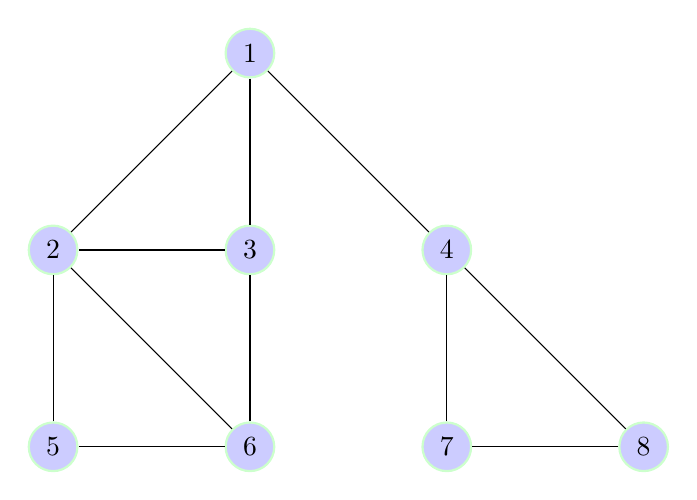
\begin{tikzpicture}{node distance=1.3cm,>=stealth',bend angle=45, auto}
        {

          \tikzstyle{place}=[circle,thick,draw=green!20,fill=blue!20,minimum size=6mm]
          \tikzstyle{texto}=[]
          \begin{scope}

            \node [place] (c1) {$2$};

            \node [place] (c2) [right of=c1,xshift=1.5cm] {$3$}
            edge [] (c1);

            \node [place] (c3) [above of=c2,yshift=1.5cm] {$1$}
            edge [] (c1)
            edge [] (c2);

            \node [place] (c4) [below of=c2,yshift=-1.5cm] {$6$}
            edge [] (c2)
            edge [] (c1);

            \node [place] (c5) [below of=c1,yshift=-1.5cm] {$5$}
            edge [] (c1)
            edge [] (c4);

            \node [place] (c6) [right of=c2,xshift=1.5cm] {$4$}
            edge [] (c3);

            \node [place] (c7) [below of=c6,yshift=-1.5cm] {$7$}
            edge [] (c6);

            \node [place] (c8) [right of=c7,xshift=1.5cm] {$8$}
            edge [] (c7)
            edge [] (c6);


          \end{scope}
        }
        \end{tikzpicture}
      \end{minipage}}
      \begin{center}
      \vspace{-2.5in}{\begin{minipage}{.05\columnwidth}%
        \centering%
        \begin{tikzpicture}{node distance=1.3cm,>=stealth',bend angle=45, auto}
          {

            \tikzstyle{place}=[circle,thick,draw=green!20,fill=blue!20,minimum size=6mm]
            \tikzstyle{texto}=[]
            \begin{scope}

              \node [place] (c1) [label=left:\textcolor{black}{$2$},label=right:\textcolor{black}{$1$}]{$2$};

              \node [texto] (c2) [right of=c1,xshift=1.5cm] {};

              \node [place] (c3) [above of=c2,yshift=1.5cm,label=right:\textcolor{black}{$1$},label=left:\textcolor{black}{$1$}] {$1$}
              edge [post] (c1);

              \node [place] (c4) [below of=c1,yshift=-.5cm,label=right:\textcolor{black}{$1$},label=left:\textcolor{black}{$3$}] {$3$}
              edge [pre] (c1)
              edge [bend right,dashed] (c3) ;

              \node [place] (c5) [below of=c4,yshift=-.5cm,label=right:\textcolor{black}{$2$},label=left:\textcolor{black}{$4$}] {$6$}
              edge [pre] (c4)
              edge [bend left=60,dashed] (c1) ;

              \node [place] (c6) [right of=c2,xshift=1.5cm,label=right:\textcolor{black}{$6$},label=left:\textcolor{black}{$6$}] {$4$}
              edge [pre] (c3);

              \node [place] (c7) [below of=c6,yshift=-.5cm,label=right:\textcolor{black}{$6$},label=left:\textcolor{black}{$7$}] {$7$}
              edge [pre] (c6);

              \node [place] (c8) [below of=c5,yshift=-.5cm,label=right:\textcolor{black}{$2$},label=left:\textcolor{black}{$5$}] {$5$}
              edge [pre] (c5)
              edge [bend left=65,dashed] (c1) ;

              \node [place] (c9) [below of=c7,yshift=-.5cm,label=right:\textcolor{black}{$6$},label=left:\textcolor{black}{$8$}] {$8$}
              edge [pre] (c7)
              edge [bend right=60,dashed] (c6) ;
            \end{scope}
          }
        \end{tikzpicture}
      \end{minipage}}
    \end{center}
  \end{figure}%
\end{center}%
\begin{figure}[H]
\caption{Un grafo no dirigido y su árbol de recorrido en profundidad.}
\end{figure}


\subsection{Búsqueda en anchura (Breadth-First Search)}

Cuando un recorrido en profundidad llega a un vértice $v$, intenta a continuación visitar algún vecino de $v$, después algún vecino del vecino, y así sucesivamente. Cuando un recorrido en anchura llega a algún vértice $v$, por otra parte, primero visita todos los vecinos de $v$. Sólo examina vértices más alejados después de haber hecho esto. A diferencia del recorrido en profundidad, el recorrido en anchura no es naturalmente recursivo.\\

Supongamos que queremos encontrar un camino más corto entre dos vértices específicos de un grafo - un camino que conecte a los vértices con la peculiaridad de que no exista otro camino con esos vértices y menos aristas. El método clásico para llevar a cabo esta tarea, llamado Búsqueda en Anchura (Breadth-First search), es también la base de numerosos algoritmos para el procesamiento de grafos. La Búsqueda en Profundidad nos ofrece poca ayuda en la resolución de este problema, ya que el orden en el que navega a través del grafo no tiene relación con el objetivo de encontrar los caminos más cortos. Por el contrario, la Búsqueda en Anchura se basa en este cometido. Para encontrar un camino más corto desde $v$ hasta $w$, que comenzará en $v$ hasta $w$ comprobando entre todos los vértices que podemos llegar siguiendo una de las aristas, luego de comprobar todos los vértices que se pueden recorrer de esos extremos y así sucesivamente.\\

Cuando llegamos a un punto de la búsqueda en el grafo en donde tenemos que atravesar más de una arista, se elige una y almacenamos las demás sin procesar para un análisis posterior. En la Búsqueda en Profundidad, se suele utilizar la inserción de elementos en una pila (que es gestionada por una función o estructura auxiliar a la función de búsqueda recursiva) para este propósito. Usando la regla LIFO que caracteriza a las pilas para explorar pasadizos o pasajes que estén muy próximos en un laberinto: Para ello elegimos, de las caminos que aún no hayan sido revisados, aquella que sea la más recientemente visitada. En la Búsqueda por Anchura, se explorarán los vértices según su ponderación o coste desde el punto de partida del camino o análisis. Para un laberinto, hacer esta búsqueda en este orden puede requerir un equipo entero de búsqueda; pero dentro de un programa de ordenador es más fácil de solucionar. Simplemente utilizaremos una estructura de tipo FIFO (cola) en lugar de una LIFO (pila).\\

\vfill
\pagebreak
\figuratikz{1}{Un árbol de búsqueda en anchura. Los nodos son numerados en el orden en que serán procesados por el algoritmo. El hijo de un nodo se visita de izquierda a derecha.}
{
  \tikzstyle{place}=[circle,thick,draw=green!20,fill=blue!20,minimum size=6mm]
  \tikzstyle{texto}=[]

  \begin{scope}

    \node [place] (c1) {$2$};

    \node [texto] (c2) [right of=c1,xshift=2.5cm] {};

    \node [place] (c3) [above of=c2,yshift=1.5cm] {$1$}
    edge [] (c1);

    \node [place] (c4) [below of=c1,yshift=-.5cm] {$6$}
    edge [] (c1);

    \node [place] (c6) [right of=c2,xshift=2.5cm] {$4$}
    edge [] (c3);

    \node [place] (c7) [below of=c6,yshift=-.5cm] {$11$}
    edge [] (c6);

    \node [place] (c10) [below of=c3,yshift=-1.5cm] {$3$}
    edge [] (c3);

    \node [place] (c11) [below of=c10,xshift=-.75cm,yshift=-.5cm] {$8$}
    edge [] (c10);

    \node [place] (c12) [below of=c10,xshift=.75cm,yshift=-.5cm] {$9$}
    edge [] (c10);

    \node [place] (c13) [left of=c4,xshift=-.25cm] {$5$}
    edge [] (c1);

    \node [place] (c14) [right of=c4,xshift=.25cm] {$7$}
    edge [] (c1);

    \node [place] (c15) [below of=c4,xshift=-.75cm,yshift=-.5cm] {$13$}
    edge [] (c4);

    \node [place] (c16) [below of=c4,xshift=.75cm,yshift=-.5cm] {$14$}
    edge [] (c4);

    \node [place] (c17) [below of=c7,xshift=-.75cm,yshift=-.5cm] {$15$}
    edge [] (c7);

    \node [place] (c17) [below of=c7,xshift=.75cm,yshift=-.5cm] {$16$}
    edge [] (c7);

  \end{scope}

}

\underline{Algoritmo de Búsqueda en Anchura}\\
\begin{Verbatim}[commandchars=\\\{\}]
\PY{c+cm}{/**}
\PY{c+cm}{ * Método observador.}
\PY{c+cm}{ * Muestra por la salida estándar el recorrido en anchura del grafo G.}
\PY{c+cm}{ * @param G matriz de adyacencia del grafo conexo.}
\PY{c+cm}{ */}

\PY{k+kd}{public} \PY{k+kt}{void} \PY{n+nf}{recorrido\PYZus{}anchura}\PY{o}{(}\PY{k+kt}{int} \PY{o}{[}\PY{o}{]}\PY{o}{[}\PY{o}{]} \PY{n}{G}\PY{o}{)} 
\PY{o}{\PYZob{}}
    \PY{k+kt}{int} \PY{n}{tama\PYZus{}G} \PY{o}{=} \PY{n}{G}\PY{o}{.}\PY{n+na}{length}\PY{o}{;}

    \PY{k+kt}{boolean} \PY{o}{[}\PY{o}{]} \PY{n}{marcas} \PY{o}{=} \PY{k}{new} \PY{k+kt}{boolean} \PY{o}{[}\PY{n}{tama\PYZus{}G}\PY{o}{]}\PY{o}{;}
    \PY{k+kt}{int} \PY{n}{i}\PY{o}{,}\PY{n}{v}\PY{o}{,}\PY{n}{w}\PY{o}{;} \PY{c+c1}{//Vértices.}

    \PY{n}{LinkedList}\PY{o}{<}\PY{n}{Integer}\PY{o}{>} \PY{n}{Cola} \PY{o}{=} \PY{k}{new} \PY{n}{LinkedList}\PY{o}{(}\PY{o}{)}\PY{o}{;}
    \PY{n}{rec\PYZus{}breadth} \PY{o}{=} \PY{k}{new} \PY{n}{ArrayList}\PY{o}{<}\PY{n}{Integer}\PY{o}{>}\PY{o}{(}\PY{o}{)}\PY{o}{;}

    \PY{n}{Arrays}\PY{o}{.}\PY{n+na}{fill}\PY{o}{(}\PY{n}{marcas}\PY{o}{,}\PY{l+m+mi}{0}\PY{o}{,}\PY{n}{tama\PYZus{}G}\PY{o}{,}\PY{k+kc}{false}\PY{o}{)}\PY{o}{;}
    \PY{n}{System}\PY{o}{.}\PY{n+na}{out}\PY{o}{.}\PY{n+na}{println}\PY{o}{(}\PY{l+s}{"REC\PYZus{}ANCHURA"}\PY{o}{)}\PY{o}{;}
    \PY{k}{for}\PY{o}{(}\PY{n}{i}\PY{o}{=}\PY{l+m+mi}{0}\PY{o}{;} \PY{n}{i} \PY{o}{<} \PY{n}{tama\PYZus{}G}\PY{o}{;} \PY{o}{+}\PY{o}{+}\PY{n}{i}\PY{o}{)}
	\PY{k}{if}\PY{o}{(}\PY{o}{!}\PY{n}{marcas}\PY{o}{[}\PY{n}{i}\PY{o}{]}\PY{o}{)} \PY{c+c1}{//NO visitado}
	    \PY{o}{\PYZob{}}
		\PY{n}{Cola}\PY{o}{.}\PY{n+na}{add}\PY{o}{(}\PY{n}{i}\PY{o}{)}\PY{o}{;} \PY{c+c1}{//Frente de la Cola}
		    
		\PY{k}{do}\PY{o}{\PYZob{}}
		    \PY{n}{v} \PY{o}{=} \PY{n}{Cola}\PY{o}{.}\PY{n+na}{getFirst}\PY{o}{(}\PY{o}{)}\PY{o}{;}
		    \PY{n}{Cola}\PY{o}{.}\PY{n+na}{removeFirst}\PY{o}{(}\PY{o}{)}\PY{o}{;} \PY{c+c1}{//Eliminamos el elemento.}
		    \PY{k}{if}\PY{o}{(}\PY{o}{!}\PY{n}{marcas}\PY{o}{[}\PY{n}{v}\PY{o}{]}\PY{o}{)} \PY{c+c1}{//NO visitado.}
			\PY{o}{\PYZob{}}
			    \PY{c+cm}{/* Marcar y procesar. */}
			    \PY{n}{marcas}\PY{o}{[}\PY{n}{v}\PY{o}{]} \PY{o}{=} \PY{k+kc}{true}\PY{o}{;} \PY{c+c1}{//Visitado.}
			    \PY{n}{System}\PY{o}{.}\PY{n+na}{out}\PY{o}{.}\PY{n+na}{print}\PY{o}{(}\PY{n}{v}\PY{o}{+}\PY{l+s}{" "}\PY{o}{)}\PY{o}{;}
			    \PY{n}{rec\PYZus{}breadth}\PY{o}{.}\PY{n+na}{add}\PY{o}{(}\PY{n}{v}\PY{o}{)}\PY{o}{;}
				
			    \PY{c+cm}{/* Encolar los adyacentes no visitados. */}

			    \PY{k}{for}\PY{o}{(}\PY{n}{w}\PY{o}{=}\PY{l+m+mi}{0}\PY{o}{;} \PY{n}{w} \PY{o}{<} \PY{n}{tama\PYZus{}G}\PY{o}{;} \PY{o}{+}\PY{o}{+}\PY{n}{w}\PY{o}{)}
				\PY{k}{if}\PY{o}{(}\PY{n}{G}\PY{o}{[}\PY{n}{v}\PY{o}{]}\PY{o}{[}\PY{n}{w}\PY{o}{]} \PY{o}{=}\PY{o}{=} \PY{l+m+mi}{1} \PY{o}{&}\PY{o}{&} \PY{n}{marcas}\PY{o}{[}\PY{n}{w}\PY{o}{]} \PY{o}{=}\PY{o}{=} \PY{k+kc}{false}\PY{o}{)}
				    \PY{n}{Cola}\PY{o}{.}\PY{n+na}{add}\PY{o}{(}\PY{n}{w}\PY{o}{)}\PY{o}{;}
			\PY{o}{\PYZcb{}}
		\PY{o}{\PYZcb{}}\PY{k}{while}\PY{o}{(}\PY{o}{!}\PY{o}{(}\PY{n}{Cola}\PY{o}{.}\PY{n+na}{isEmpty}\PY{o}{(}\PY{o}{)}\PY{o}{)}\PY{o}{)}\PY{o}{;}
	    \PY{o}{\PYZcb{}}
    \PY{n}{System}\PY{o}{.}\PY{n+na}{out}\PY{o}{.}\PY{n+na}{println}\PY{o}{(}\PY{l+s}{""}\PY{o}{)}\PY{o}{;}
\PY{o}{\PYZcb{}}
\end{Verbatim}


\section{Coloración}

En ocasiones, un problema se puede modelar distribuyendo los vértices o las aristas de un cierto grafo en paquetes distintos, de manera que vértices (o aristas, en su caso) de un mismo paquete no sean adyacentes (respectivamente, incidentes). Si se da un mismo color a los elementos de un mismo paquete, y se emplean colores distintos para cada paquete, se obtiene lo que se da en llamar un vértice (arista) coloración. La idea es encontrar el menor número de paquetes (esto es, colores), para distribuir los elementos (vértices o aristas, según sea el caso).\\

Un planteamiento general que se ajusta a esta circunstancia es el llamado \emph{problema de incompatibilidades}, que consta de ciertos elementos (modelados por los vértices de un grafo) y relaciones de incompatibilidad entre ellos (las cuales determinan las aristas del grafo). El grafo resultante se denomina \emph{grafo de incompatibilidades}. El distribuir los elementos en el menor número de agrupaciones posible de forma que elementos incompatibles no compartan una misma agrupación, se traduce al instante en conseguir una vértice coloración (i.e.\footnote{Del Latín i.e. ``id est'' Significado: ``Esto es'', ``Es decir''} una asignación de colores a los vértices de manera que vértices adyacentes tengan colores distintos).\\

Como ejemplo, se puede considerar el problema de diseñar un calendario a doble vuelta para una competición deportiva en forma de liguilla de $n$ equipos, en la que todos se han de enfrentar con todos dos veces. Este problema admite una primera simplificación, en la que basta diseñar un calendario a una sola vuelta, para reproducirlo en la segunda vuelta cambiando los papeles de los equipos que juegan como locales y como visitantes.\\

Si se modela el problema como el grafo $G$ cuyos vértices son los $n$ equipos y las aristas entre ellos representan los partidos, evidentemente se tiene que $G = K_n$, grafo completo de $n$ vértices. Organizar el calendario se traduce en repartir los partidos (aristas) en jornadas (colores), de manera que un mismo equipo (vértice) no juegue más de una vez en cada jornada (no aparezca como extremo en más de una arista). En definitiva, se trata de colorear las aristas de $K_n$ utilizando el menor número de colores, de manera que aristas con el mismo color representan partidos que se pueden jugar en la misma jornada.\\

Este problema admite ser modelado de otra forma: considérese el grafo $H$ cuyos vértices son los partidos a jugar, y cuyas aristas relacionan partidos incompatibles, en tanto en cuanto implican a un mismo equipo. Resolver el problema consiste ahora en encontrar una vértice coloración de $H$.\\

\subsection{Vértice coloraciones}

\begin{fondo}
Se denomina vértice coloración de un grafo $G = (V,A)$ a una asignación $c: V \rightarrow \mathbb{N}$ que asocie a cada vértice $x_i$ un color $c_i \in \mathbb{N}$, de manera que a vértices adyacentes correspondan colores distintos: si $\{x_i,x_j\} \in A$ entonces $c_i \ne c_j$. Si la coloración consta de una paleta de $k$ colores, entonces se habla simplemente de $k$-coloración.
\end{fondo}

Dado un grafo $G = (V,A)$, siempre existe un valor umbral $k$ para el cual $G$ admite una vértice coloración con una paleta de $k$ colores, pero no una $(k-1)$-coloración. Es decir, $k$ es el menor número de colores con los que se puede obtener una vértice coloración de $G$. Este valor se conoce como \emph{número cromático} de $G$, y se denota en la forma $\chi (G) = k$.\\

Determinar cuál es el número cromático de un grafo es en general un problema de una envergadura considerable: \textbf{no hay} un procedimiento que dé una respuesta en tiempo razonable, para un grafo genérico dado.\\

Ni que decir tiene que el número cromático de un grafo no conexo consiste en el mayor de entre los números cromáticos de sus componentes conexas, razón por la cual nos centraremos en el estudio de coloraciones sobres grafos conexos.\\

Con normalidad, se tiende a acotar el número cromático tanto inferior como superiormente, $s \leq \chi (G) \leq t$, de manera que progresivamente se afinan estas cotas hasta llevarlas a coincidir, $s = \chi (G) = t$, momento en el cual queda completamente determinado $\chi (G)$.\\

Sin mucho esfuerzo, es fácil asegurar de entrada que $1 \leq \chi (G) \leq v$ para grafos $G$ de $v$ vértices. Más aún, $\chi (G) = 1$ sólo en el caso de grafos $G$ vacíos, mientras que $\chi (G) = v$ en un grafo de $v$ vértices sólo si $G = K_v$.\\

El \textbf{teorema de Brooks} perfila un poco más la cota superior para $\chi (G)$ en grafos conexos, en función de la valencia (grado) máxima:
\[ \Delta =\ \mbox{max}_{x \in V}\ gr_G(x):
\left\{ 
\begin{array}{l}
\chi (K_n) = n = \Delta + 1\ \mbox{y}\ \chi (C_{2n + 1}) = 3 = \Delta + 1 \\
\mbox{En otro caso,}\ \chi (G) \leq \Delta
\end{array}
\right. \]

No obstante, esta cota puede ser bastante rudimentaria (piénsese en un grafo estrella $S_m$ de $m$ puntas, con $m = 1000$ por ejemplo: se tiene que $\chi (S_m) = 2$, mientras que $\Delta = m = 1000$).\\

Para obtener cotas inferiores, es frecuente buscar subgrafos $H \subseteq G$ de los cuales se conozca $\chi (H)$, toda vez que $\chi (H) \leq \chi (G)$ para cualquier $H \subseteq G$.\\

Para obtener cotas superiores, se suele realizar coloraciones concretas, de manera que $\chi (G)$ siempre es menor o igual que el número de colores utilizados.\\

A la hora de realizar coloraciones, es útil el llamado \emph{algoritmo voraz}, el cual, progresando sobre una ordenación prefijada de los vértices, procede a colorearlos asignando a cada vértice el primer color libre (i.e. el primer color no utilizado en los vértices a él adyacentes previamente coloreados).\\

Aunque este algoritmo no tiene por qué devolver el número cromático de $G$, con normalidad devuelve un número razonablemente pequeño de colores. No obstante, siempre se puede aplicar varias veces el algoritmo a ordenaciones distintas de los vértices, para ver si eventualmente el número de colores desciende. Una aplicación exhaustiva del algoritmo a las $V!$ ordenaciones posibles en un grafo de $V$ vértices resolvería efectivamente el problema; la ``única'' dificultad estriba en que $V!$ aplicaciones del algoritmo resultan ya impracticables cuando $V$ no es siquiera demasiado grande (nótese que $8! = 40320$).\\

\underline{Algoritmo de Vértice Coloración (Número Cromático)}\\
\begin{Verbatim}[commandchars=\\\{\}]
\PY{c+cm}{/**}
\PY{c+cm}{ * Método observador (Número cromático del grafo)}
\PY{c+cm}{ * @param G: matriz bidimensional de enteros que representa al grafo de}
\PY{c+cm}{ * trabajo actual.}
\PY{c+cm}{ * @return int que es el número cromático del grafo.}
\PY{c+cm}{ */}

\PY{k+kd}{public} \PY{k+kt}{int} \PY{n+nf}{k\PYZus{}colores}\PY{o}{(}\PY{k+kt}{int} \PY{o}{[}\PY{o}{]}\PY{o}{[}\PY{o}{]} \PY{n}{G}\PY{o}{)}
\PY{o}{\PYZob{}}
    \PY{k+kt}{int} \PY{n}{tama\PYZus{}G} \PY{o}{=} \PY{n}{G}\PY{o}{.}\PY{n+na}{length}\PY{o}{;}
    \PY{k+kt}{int} \PY{n}{elto}\PY{o}{=}\PY{l+m+mi}{0}\PY{o}{,} \PY{n}{original}\PY{o}{=}\PY{l+m+mi}{0}\PY{o}{;}
    \PY{k+kt}{int} \PY{o}{[}\PY{o}{]} \PY{n}{color} \PY{o}{=} \PY{k}{new} \PY{k+kt}{int} \PY{o}{[}\PY{n}{tama\PYZus{}G}\PY{o}{]}\PY{o}{;}
    \PY{n}{Arrays}\PY{o}{.}\PY{n+na}{fill}\PY{o}{(}\PY{n}{color}\PY{o}{,}\PY{l+m+mi}{0}\PY{o}{)}\PY{o}{;} \PY{c+c1}{//Rellenamos con el color vacío todo el vector.}
    \PY{k+kt}{int} \PY{n}{i}\PY{o}{;}
    \PY{k+kt}{boolean} \PY{n}{salto}\PY{o}{=}\PY{k+kc}{false}\PY{o}{;}


    \PY{n}{HashMap}\PY{o}{<}\PY{n}{Integer}\PY{o}{,}\PY{n}{ArrayList}\PY{o}{<}\PY{n}{Integer}\PY{o}{>}\PY{o}{>}  \PY{n}{v\PYZus{}ady} 
	\PY{o}{=} \PY{k}{new} \PY{n}{HashMap}\PY{o}{<}\PY{n}{Integer}\PY{o}{,}\PY{n}{ArrayList}\PY{o}{<}\PY{n}{Integer}\PY{o}{>}\PY{o}{>}\PY{o}{(}\PY{o}{)}\PY{o}{;}
    \PY{n}{ArrayList}\PY{o}{<}\PY{n}{Integer}\PY{o}{>} \PY{n}{ady}\PY{o}{;}


    \PY{k}{for}\PY{o}{(}\PY{n}{i}\PY{o}{=}\PY{l+m+mi}{0}\PY{o}{;} \PY{n}{i} \PY{o}{<} \PY{n}{tama\PYZus{}G}\PY{o}{;} \PY{o}{+}\PY{o}{+}\PY{n}{i}\PY{o}{)}
	\PY{o}{\PYZob{}}
	    \PY{n}{ady} \PY{o}{=} \PY{k}{new} \PY{n}{ArrayList}\PY{o}{<}\PY{n}{Integer}\PY{o}{>}\PY{o}{(}\PY{o}{)}\PY{o}{;}

	    \PY{k}{for}\PY{o}{(}\PY{k+kt}{int} \PY{n}{j}\PY{o}{=}\PY{l+m+mi}{0}\PY{o}{;} \PY{n}{j} \PY{o}{<} \PY{n}{tama\PYZus{}G}\PY{o}{;} \PY{o}{+}\PY{o}{+}\PY{n}{j}\PY{o}{)}
		\PY{o}{\PYZob{}}
		    \PY{k}{if}\PY{o}{(}\PY{n}{G}\PY{o}{[}\PY{n}{i}\PY{o}{]}\PY{o}{[}\PY{n}{j}\PY{o}{]} \PY{o}{!}\PY{o}{=} \PY{l+m+mi}{0}\PY{o}{)}
			\PY{o}{\PYZob{}}
			    \PY{n}{ady}\PY{o}{.}\PY{n+na}{add}\PY{o}{(}\PY{n}{j}\PY{o}{)}\PY{o}{;}
			\PY{o}{\PYZcb{}}
		\PY{o}{\PYZcb{}}

	    \PY{n}{v\PYZus{}ady}\PY{o}{.}\PY{n+na}{put}\PY{o}{(}\PY{n}{i}\PY{o}{,}\PY{n}{ady}\PY{o}{)}\PY{o}{;}
	\PY{o}{\PYZcb{}}

    \PY{n}{i}\PY{o}{=}\PY{l+m+mi}{0}\PY{o}{;}
    \PY{k+kt}{int} \PY{n}{z}\PY{o}{=}\PY{l+m+mi}{0}\PY{o}{;}
    \PY{k}{while}\PY{o}{(}\PY{n}{i} \PY{o}{<} \PY{n}{tama\PYZus{}G}\PY{o}{)}
	\PY{o}{\PYZob{}}
	    \PY{n}{z} \PY{o}{=} \PY{n}{rec\PYZus{}depth}\PY{o}{.}\PY{n+na}{get}\PY{o}{(}\PY{n}{i}\PY{o}{)}\PY{o}{;}
	    \PY{n}{color}\PY{o}{[}\PY{n}{z}\PY{o}{]} \PY{o}{+}\PY{o}{=} \PY{l+m+mi}{1}\PY{o}{;}
	    \PY{n}{original} \PY{o}{=} \PY{n}{color}\PY{o}{[}\PY{n}{z}\PY{o}{]}\PY{o}{;}

	    \PY{k}{for}\PY{o}{(}\PY{k+kt}{int} \PY{n}{j}\PY{o}{=}\PY{l+m+mi}{0}\PY{o}{;} \PY{n}{j} \PY{o}{<} \PY{n}{v\PYZus{}ady}\PY{o}{.}\PY{n+na}{get}\PY{o}{(}\PY{n}{z}\PY{o}{)}\PY{o}{.}\PY{n+na}{size}\PY{o}{(}\PY{o}{)} \PY{o}{&}\PY{o}{&} \PY{o}{!}\PY{n}{salto}\PY{o}{;} \PY{o}{+}\PY{o}{+}\PY{n}{j}\PY{o}{)}
		\PY{o}{\PYZob{}}
		    \PY{n}{elto} \PY{o}{=} \PY{n}{v\PYZus{}ady}\PY{o}{.}\PY{n+na}{get}\PY{o}{(}\PY{n}{z}\PY{o}{)}\PY{o}{.}\PY{n+na}{get}\PY{o}{(}\PY{n}{j}\PY{o}{)}\PY{o}{;}
		    \PY{k}{if}\PY{o}{(}\PY{n}{color}\PY{o}{[}\PY{n}{elto}\PY{o}{]} \PY{o}{=}\PY{o}{=} \PY{n}{color}\PY{o}{[}\PY{n}{z}\PY{o}{]}\PY{o}{)}
			\PY{o}{\PYZob{}}
			    \PY{n}{color}\PY{o}{[}\PY{n}{z}\PY{o}{]} \PY{o}{+}\PY{o}{=} \PY{l+m+mi}{1}\PY{o}{;}
			    \PY{n}{salto} \PY{o}{=} \PY{k+kc}{true}\PY{o}{;}
			\PY{o}{\PYZcb{}}
		\PY{o}{\PYZcb{}}

       
	    \PY{k}{if}\PY{o}{(}\PY{n}{original} \PY{o}{=}\PY{o}{=} \PY{n}{color}\PY{o}{[}\PY{n}{z}\PY{o}{]}\PY{o}{)}
		\PY{n}{i}\PY{o}{+}\PY{o}{+}\PY{o}{;}
	    \PY{k}{else}
		\PY{n}{i}\PY{o}{=}\PY{l+m+mi}{0}\PY{o}{;}
	\PY{o}{\PYZcb{}} 

    \PY{n}{elto} \PY{o}{=} \PY{n}{color}\PY{o}{[}\PY{l+m+mi}{0}\PY{o}{]}\PY{o}{;}
	
    \PY{k}{for}\PY{o}{(}\PY{n}{i}\PY{o}{=}\PY{l+m+mi}{0}\PY{o}{;} \PY{n}{i} \PY{o}{<} \PY{n}{tama\PYZus{}G}\PY{o}{;} \PY{o}{+}\PY{o}{+}\PY{n}{i}\PY{o}{)}
	\PY{k}{if}\PY{o}{(}\PY{n}{color}\PY{o}{[}\PY{n}{i}\PY{o}{]} \PY{o}{>} \PY{n}{elto}\PY{o}{)}
	    \PY{n}{elto} \PY{o}{=} \PY{n}{color}\PY{o}{[}\PY{n}{i}\PY{o}{]}\PY{o}{;}

    \PY{k}{return} \PY{n}{elto}\PY{o}{;}

	
\PY{o}{\PYZcb{}}
\end{Verbatim}


\section{Ordenación topológica}

La Ordenación Topológica es la operación más importante en los grafos acíclicos dirigidos (DAG). Este ordena los vértices en una línea de tal manera que todas las aristas dirigidas vayan de izquierda a derecha. Tal ordenamiento no puede existir si el grafo contiene un ciclo dirigido.\\

Cada DAG tiene al menos una ordenación topológica. La importancia de la ordenación topológica es que ordena procesando cada vértice antes de cualquier sucesor que tenga. Supongamos que las aristas representan restricciones de prioridad, de modo que la arista $(x,y)$ significa que el trabajo o proceso $x$ debe hacerse antes del proceso $y$. Entonces, cualquier ordenación topológica define un programa de forma lícita. De hecho, puede haber muchas ordenaciones para un mismo DAG dado.\\

\figuratikz{1}{Un DAG con un solo orden topológico $(G,A,B,C,F,E,D)$}
{
  \tikzstyle{place}=[circle,thick,draw=green!20,fill=blue!20,minimum size=4mm]

  \begin{scope}

    \node [place] (c1) [label=left:\textcolor{black}{$A$}] {};

    \node [place] (c2) [below of=c1,yshift=-1cm,label=left:\textcolor{black}{$G$}] {}
    edge [post] (c1);

    \node [place] (c3) [right of=c1,xshift=.5cm,yshift=.5cm,label=above:\textcolor{black}{$B$}] {}
    edge [pre] (c1);

    \node [place] (c4) [below of=c3,yshift=-.2cm,xshift=.4cm,label=below:\textcolor{black}{$C$}] {}
    edge [pre] (c3)
    edge [pre] (c1);

    \node [place] (c5) [right of=c2,xshift=3cm,label=right:\textcolor{black}{$F$}] {}
    edge [pre] (c2)
    edge [pre] (c4);

    \node [place] (c6) [right of=c4,xshift=1cm,yshift=.3cm,label=right:\textcolor{black}{$E$}] {}
    edge [pre] (c4)
    edge [pre] (c5);

    \node [place] (c7) [right of=c6,xshift=.4cm,yshift=.8cm,label=above:\textcolor{black}{$D$}] {}
    edge [pre] (c3)
    edge [pre] (c6);


  \end{scope}

}

Pero las aplicaciones son más variadas. Supongamos que buscamos el camino más corto (o largo) desde $x$ a $y$ en un DAG. Ningún vértice aparece después de $y$ en el orden topológico que puede contribuir a cualquiera de estos caminos, porque no habrá forma de volver a $y$. Podríamos procesar de forma correcta todos los vértices desde la izquierda a la derecha en el orden topológico, considerando el impacto de sus aristas exteriores, y sabiendo que se han analizado todo antes de que se necesite en otra operación. El orden topológico resulta muy útil para prácticamente cualquier problema algorítmico en grafos dirigidos.\\

El orden topológico puede realizarse de una manera eficiente usando la búsqueda en profundidad. Un grafo dirigido es un DAG si y sólo si no hay aristas de retroceso en él. Etiquetando los vértices en el orden inverso al que fueron procesados se encuentra una ordenación topológica de un DAG. ¿Porqué? Considere que sucede con cada arista dirigida $\{x,y\}$ cuando nos encontramos explorando el vértice $x$:\\

\begin{itemize}
\item Si no se ha pasado por $y$ aún, entonces comenzaremos una búsqueda en profundidad en $y$ antes de que podamos continuar con $x$. Por lo tanto, $y$ es marcado como "procesado" antes que $x$ lo sea, y $x$ aparece antes que $y$ en la ordenación topológica, como debería ser.
\item Si se ha pasado por $y$ pero no se ha marcado como "procesado", entonces $\{x,y\}$ es una arista de retroceso, lo cual no estaría permitido en un DAG.
\item Si $y$ se ha procesado, entonces habrá sido etiquetado antes que $x$. De tal forma que, $x$ aparece antes que $y$ en el orden topológico, como debería ser
\end{itemize}

\underline{Algoritmo de Ordenación Topológica}\\
\begin{Verbatim}[commandchars=\\\{\}]
\PY{c+cm}{/**}
\PY{c+cm}{ * Método modificador }
\PY{c+cm}{ * Realiza la ordenación topológica del grafo de trabajo y la muestra}
\PY{c+cm}{ * por el flujo de salida estándar.}
\PY{c+cm}{ * @param G: matriz bidimensional de enteros cuyo contenido es el grafo}
\PY{c+cm}{ * de trabajo actual.}
\PY{c+cm}{ */}

\PY{k+kd}{public} \PY{k+kt}{void} \PY{n+nf}{ordenacion\PYZus{}topologica}\PY{o}{(}\PY{k+kt}{int} \PY{o}{[}\PY{o}{]}\PY{o}{[}\PY{o}{]} \PY{n}{G}\PY{o}{)}
\PY{o}{\PYZob{}}
    \PY{n}{System}\PY{o}{.}\PY{n+na}{out}\PY{o}{.}\PY{n+na}{println}\PY{o}{(}\PY{l+s}{"ORDENACION TOPOLOGICA"}\PY{o}{)}\PY{o}{;}
	
    \PY{k+kt}{int} \PY{n}{tama\PYZus{}G} \PY{o}{=} \PY{n}{G}\PY{o}{.}\PY{n+na}{length}\PY{o}{;}
    \PY{n}{vertice\PYZus{}visitado} \PY{o}{=} \PY{k}{new} \PY{k+kt}{boolean} \PY{o}{[}\PY{n}{tama\PYZus{}G}\PY{o}{]}\PY{o}{;}
    \PY{n}{pila} \PY{o}{=} \PY{k}{new} \PY{n}{Stack}\PY{o}{<}\PY{n}{Integer}\PY{o}{>}\PY{o}{(}\PY{o}{)}\PY{o}{;}

    \PY{k}{for}\PY{o}{(}\PY{k+kt}{int} \PY{n}{i}\PY{o}{=}\PY{l+m+mi}{0}\PY{o}{;} \PY{n}{i} \PY{o}{<} \PY{n}{tama\PYZus{}G}\PY{o}{;} \PY{o}{+}\PY{o}{+}\PY{n}{i}\PY{o}{)}
	\PY{n}{vertice\PYZus{}visitado}\PY{o}{[}\PY{n}{i}\PY{o}{]} \PY{o}{=} \PY{k+kc}{true}\PY{o}{;}

    \PY{k}{for}\PY{o}{(}\PY{k+kt}{int} \PY{n}{i}\PY{o}{=}\PY{l+m+mi}{0}\PY{o}{;} \PY{n}{i} \PY{o}{<} \PY{n}{tama\PYZus{}G}\PY{o}{;} \PY{o}{+}\PY{o}{+}\PY{n}{i}\PY{o}{)}
	\PY{k}{if}\PY{o}{(}\PY{n}{vertice\PYZus{}visitado}\PY{o}{[}\PY{n}{i}\PY{o}{]}\PY{o}{)}
	    \PY{n}{topolog\PYZus{}rec}\PY{o}{(}\PY{n}{i}\PY{o}{,}\PY{n}{G}\PY{o}{)}\PY{o}{;}

    \PY{n}{Stack}\PY{o}{<}\PY{n}{Integer}\PY{o}{>} \PY{n}{salida} \PY{o}{=} \PY{k}{new} \PY{n}{Stack}\PY{o}{<}\PY{n}{Integer}\PY{o}{>}\PY{o}{(}\PY{o}{)}\PY{o}{;}

    \PY{k}{while}\PY{o}{(}\PY{o}{!}\PY{n}{pila}\PY{o}{.}\PY{n+na}{empty}\PY{o}{(}\PY{o}{)}\PY{o}{)}
	\PY{o}{\PYZob{}}
	    \PY{n}{salida}\PY{o}{.}\PY{n+na}{push}\PY{o}{(}\PY{n}{pila}\PY{o}{.}\PY{n+na}{peek}\PY{o}{(}\PY{o}{)}\PY{o}{)}\PY{o}{;}
	    \PY{n}{pila}\PY{o}{.}\PY{n+na}{pop}\PY{o}{(}\PY{o}{)}\PY{o}{;}
	\PY{o}{\PYZcb{}}

    \PY{n}{System}\PY{o}{.}\PY{n+na}{out}\PY{o}{.}\PY{n+na}{print}\PY{o}{(}\PY{l+s}{"("}\PY{o}{)}\PY{o}{;}
    \PY{k}{while}\PY{o}{(}\PY{o}{!}\PY{n}{salida}\PY{o}{.}\PY{n+na}{empty}\PY{o}{(}\PY{o}{)}\PY{o}{)}
	\PY{o}{\PYZob{}}
	    \PY{n}{System}\PY{o}{.}\PY{n+na}{out}\PY{o}{.}\PY{n+na}{print}\PY{o}{(}\PY{l+s}{" "}\PY{o}{+}\PY{n}{salida}\PY{o}{.}\PY{n+na}{peek}\PY{o}{(}\PY{o}{)}\PY{o}{)}\PY{o}{;}
	    \PY{n}{salida}\PY{o}{.}\PY{n+na}{pop}\PY{o}{(}\PY{o}{)}\PY{o}{;}
	\PY{o}{\PYZcb{}}
    \PY{n}{System}\PY{o}{.}\PY{n+na}{out}\PY{o}{.}\PY{n+na}{println}\PY{o}{(}\PY{l+s}{" )"}\PY{o}{)}\PY{o}{;}
\PY{o}{\PYZcb{}}

\PY{c+cm}{/**}
\PY{c+cm}{ * Método observador. (privado)}
\PY{c+cm}{ * Es la función auxiliar que ayuda a procesar el orden topológico}
\PY{c+cm}{ * para el grafo actual.}
\PY{c+cm}{ * @param G: matriz bidimensional de enteros cuyo contenido es el grafo}
\PY{c+cm}{ * de trabajo actual.}
\PY{c+cm}{ * @param vertice: valor entero que representa un nodo del grafo G.}
\PY{c+cm}{ */}

\PY{k+kd}{private} \PY{k+kt}{void} \PY{n+nf}{topolog\PYZus{}rec}\PY{o}{(}\PY{k+kt}{int} \PY{n}{vertice}\PY{o}{,} \PY{k+kt}{int} \PY{o}{[}\PY{o}{]}\PY{o}{[}\PY{o}{]} \PY{n}{G}\PY{o}{)}
\PY{o}{\PYZob{}}
    \PY{n}{vertice\PYZus{}visitado}\PY{o}{[}\PY{n}{vertice}\PY{o}{]} \PY{o}{=} \PY{k+kc}{false}\PY{o}{;}
    \PY{k+kt}{int} \PY{n}{tama\PYZus{}G} \PY{o}{=} \PY{n}{G}\PY{o}{.}\PY{n+na}{length}\PY{o}{;}

    \PY{k}{for}\PY{o}{(}\PY{k+kt}{int} \PY{n}{i}\PY{o}{=}\PY{l+m+mi}{0}\PY{o}{;} \PY{n}{i} \PY{o}{<} \PY{n}{tama\PYZus{}G}\PY{o}{;} \PY{o}{+}\PY{o}{+}\PY{n}{i}\PY{o}{)}
	\PY{k}{if}\PY{o}{(}\PY{n}{G}\PY{o}{[}\PY{n}{i}\PY{o}{]}\PY{o}{[}\PY{n}{vertice}\PY{o}{]} \PY{o}{!}\PY{o}{=} \PY{l+m+mi}{0}\PY{o}{)}
	    \PY{k}{if}\PY{o}{(}\PY{n}{vertice\PYZus{}visitado}\PY{o}{[}\PY{n}{i}\PY{o}{]}\PY{o}{)}
		\PY{n}{topolog\PYZus{}rec}\PY{o}{(}\PY{n}{i}\PY{o}{,}\PY{n}{G}\PY{o}{)}\PY{o}{;}

    \PY{n}{pila}\PY{o}{.}\PY{n+na}{push}\PY{o}{(}\PY{n}{vertice}\PY{o}{)}\PY{o}{;}
\PY{o}{\PYZcb{}}
\end{Verbatim}

